\pdfoutput=1
\documentclass[11pt]{amsart}
\usepackage{amsmath,amssymb,amsthm}
\usepackage[margin=1.2in]{geometry}
\usepackage{booktabs,adjustbox,xcolor,graphicx}
\usepackage[colorlinks=true,linkcolor=blue,citecolor=blue,urlcolor=blue]{hyperref}
\hypersetup{pdfauthor={Bernd Johannes Wuebben},
pdftitle={Hermitian--Yang--Mills flow on degenerating Calabi--Yau threefolds of type K}}
\setlength{\emergencystretch}{2em}
\newtheorem{theorem}{Theorem}[section]
\newtheorem{proposition}[theorem]{Proposition}
\newtheorem{lemma}[theorem]{Lemma}
\newtheorem{corollary}[theorem]{Corollary}
\theoremstyle{definition}
\newtheorem{definition}[theorem]{Definition}
\newtheorem{example}[theorem]{Example}
\newtheorem{question}[theorem]{Question}
\theoremstyle{remark}
\newtheorem{remark}[theorem]{Remark}
\newcommand{\RR}{\mathbb R}
\newcommand{\CC}{\mathbb C}
\newcommand{\ZZ}{\mathbb Z}
\newcommand{\PP}{\mathbb P}
\newcommand{\cE}{\mathcal E}
\newcommand{\cX}{\mathcal X}
\newcommand{\cB}{\mathcal B}
\newcommand{\cP}{\mathcal P}
\newcommand{\cF}{\mathcal F}
\newcommand{\End}{\operatorname{End}}
\newcommand{\Herm}{\operatorname{Herm}}
\newcommand{\Ad}{\operatorname{Ad}}
\newcommand{\tr}{\operatorname{tr}}
\newcommand{\id}{\operatorname{id}}
\newcommand{\SU}{\operatorname{SU}}
\newcommand{\Comm}{\operatorname{Comm}}
\newcommand{\HS}{\mathrm{HS}}
\newcommand{\op}{\mathrm{op}}
\newcommand{\Geo}{\operatorname{Geo}}
\title[HYM flow on type K threefolds]{Hermitian--Yang--Mills flow on degenerating\\Calabi--Yau threefolds of type K}
\author{Bernd Johannes Wuebben}
\subjclass[2020]{53C07 (primary); 14J32, 14D06, 58J35, 58J50 (secondary)}
\keywords{Hermitian--Yang--Mills flow, Calabi--Yau threefold, Enriques involution,
nodal degeneration, small eigenvalue, bundle gluing}
\date{November 11, 2026\\This version: November 11, 2026}

\begin{document}
\begin{abstract}
We construct a rank-four holomorphic bundle family on a compact
degeneration, with smoothing parameter $t$, of Enriques Calabi--Yau
threefolds. The threefolds are free quotients of products of a K3
surface and an elliptic curve degenerating to a cycle of four rational
curves. On the unitary gluing locus, the bundles have nonflat
Hermitian--Einstein connections for prescribed product-induced
K\"ahler metrics, which need not be Ricci-flat. We identify all five
small eigenvalues of the trace-free endomorphism Laplacian, prove
relative asymptotics uniform up to strict polystability, and establish
a uniform complementary gap. The effective quadratic energy lies on
an interval with one-dimensional endpoint constraints whose relative
angle records holonomy around the elliptic central-fibre cycle.
We derive a finite-dimensional gradient flow of noncommuting positive Hermitian
matrices and reconstruct comparison metrics approximating actual Hermitian--Yang--Mills
trajectories in global $L^2$ affine distance.
With determinant fixed to that of the Hermitian--Einstein reference metric,
an open class of initial metrics whose relative logarithms are globally
bounded and whose component-exterior restrictions admit uniformly bounded
$C^{6,\beta}$ extensions to the normalization components,
$0<\beta<1$, enters this description after physical time $s=o(L)$,
where $L=\log(1/|t|)$. Tracking is uniform on bounded $s/L$ intervals
and, where the least effective eigenvalue is bounded below by a
positive constant, for all subsequent times. Within the specified
family, the five eigenvalues, elliptic component areas and known
normalization $L$ asymptotically recover the projective conjugacy
class of the cycle transport. Infinite physical-time limits need not
commute with degeneration. The rescaled limits commute under this
gap bound when the selected parallel limits of the component flows
and the gluing parameters converge, but can fail near reducibility.
\end{abstract}
\maketitle
\section{Introduction}\label{sec:introduction}

A degeneration of the base can create slowly relaxing endomorphisms of a
Hermitian--Einstein bundle even when its connection has nonzero curvature.
The local parallel algebras, their identifications across the degenerating
regions, and the symmetries of the compact family determine which of these
endomorphisms survive globally. We study this mechanism on a compact
Calabi--Yau threefold with a nontrivial rank-four bundle. Its effective metric
variables form a five-dimensional constrained space, and the constraints
retain gluing information that the scalar dual graph of the central fibre
does not record.

Our threefolds are free quotients of a product of a fixed K3 surface and
an elliptic curve. Such Calabi--Yau threefolds are called of \emph{type K}.
Here a Calabi--Yau threefold means a smooth projective threefold with
trivial canonical bundle and $h^{1,0}=h^{2,0}=0$. The examples have infinite
fundamental group and an index-two product cover. The K\"ahler metrics used
in the analysis descend from a fixed Ricci-flat K3 metric and a smooth
ambient metric on the degenerating elliptic family. They need not be
Ricci-flat. The geometric construction, its actual bundle connection,
and these metric choices are specified in Section~\ref{sec:geometry}.

\subsection{The family and the main result}
Let $S$ be a projective K3 surface with a free Enriques involution
$\iota$. Resolve the two successive singular points of
\[
 y^2z=x(x-z)(x-t^2z)
\]
over $t=0$. This gives a projective elliptic family $\cE\to\Delta$
with central fibre a cycle of four rational curves $D_j$, indexed
modulo four. Elliptic inversion $\sigma$ acts by $j\mapsto-j$.
Set $X_t=(S\times E_t)/\langle(\iota,\sigma)\rangle$.
The central threefold has three components, with interval dual graph.
Choose the K3 metric to have volume one. The actual elliptic
component areas are $A_0,A_1,A_2,A_3=A_1>0$.

For $\theta\in\RR$ let
\[
 R=e^{i\theta\sigma_z/4},\qquad J=i\sigma_x,
 \qquad U_\theta=R^4,
 \qquad
 \sigma_x=\begin{pmatrix}0&1\\1&0\end{pmatrix},\quad
 \sigma_z=\begin{pmatrix}1&0\\0&-1\end{pmatrix}.
\]
The rank-two flat bundle $V_\theta$ on the elliptic cover has transport
$R$ at each oriented node incidence, cycle holonomy $U_\theta$,
and trivial vanishing-cycle holonomy. Its lift of $\sigma$ has square
$-I$. Tensoring this lift with $i\,d\iota$ gives a genuine
order-two action on $T^{1,0}S\otimes V_\theta$, which descends to
a rank-four bundle $\cB_{t,\theta}$. Section~\ref{sec:geometry}
constructs these transitions on an actual cover of the compact
total space and verifies the descent. In particular, the family is
not specified merely by a proposed local gluing diagram.

Let $L=\log(1/|t|)$. On
$\RR\oplus\RR^3\oplus\RR$ define the energy and mass
\begin{equation}\label{eq:intro-forms}
 \begin{split}
 q_\theta(a,X,b)&=2\bigl(\|au-X\|^2+\|X-bv_\theta\|^2\bigr),\\
 m_A(a,X,b)&=A_0a^2+2A_1\|X\|^2+A_2b^2,\\
 u&=(1,0,0),\qquad v_\theta=(\cos\theta,\sin\theta,0).
 \end{split}
\end{equation}
Write $\mu_0\le\cdots\le\mu_4$ for their generalized eigenvalues,
including zero modes. Let $\cP_2$ be the space of positive Hermitian
two-by-two matrices of determinant one, with affine invariant metric
\eqref{eq:matrix-metric}, and let $d_2$ be its geodesic distance.
The finite-dimensional configuration space is
\[
 \cF=\{(H_j)\in\cP_2^4:H_{-j}=JH_jJ^*\},
 \qquad g_M=\sum_j A_jg_{H_j}.
\]
It is a five-dimensional geodesically convex submanifold. The two
endpoint factors are one-dimensional, whereas the middle factor
has dimension three and weight $2A_1$.

The initial tuple for the effective evolution is selected from the
spatial initial metric. On each fixed normalization component, run
the HYM metric flow and take its parallel limiting metric. We call
this limit the \emph{component phase}. It is a positive metric in
the component's parallel endomorphism algebra, rather than an angular
parameter. Theorem~\ref{thm:parallel-phase} proves its existence and
quantitative dependence on the initial metric. In the degeneration,
the component restrictions admit smooth extensions across shrinking
node discs; the allowed extensions and their asymptotically vanishing
phase ambiguity are specified in Section~\ref{sec:spatial-entry}.
The norm used there controls the logarithm of the relative metric
globally in $C^0$ and controls extensions of its component-exterior
restrictions to the fixed spaces $S\times D_j$ in $C^{6,\beta}$.
It permits spatial variation in both factors and arbitrary smooth
changes of bounded amplitude inside the middle neck regions.

\begin{theorem}\label{thm:main}
For the compact family, bundle and prescribed K\"ahler metrics just
described, the following statements hold on the same smooth fibres.
\begin{enumerate}
\item The bundle has a holomorphically trivial determinant and an
explicit determinant-normalized Hermitian--Einstein metric $h_0$.
On an embedded K3 slice its second Chern number is $48$. It is
stable for $\theta\notin\pi\ZZ$ and strictly polystable for
$\theta\in\pi\ZZ$.
\item Let $\lambda_k(t,\theta)$ be the eigenvalues, indexed from
zero, of the actual endomorphism connection Laplacian
$D_\theta^*D_\theta$ on trace-free $h_0$-Hermitian endomorphisms.
There are $\varepsilon(t)\to0$ and $\gamma>0$, independent of
$\theta$, such that
\begin{equation}\label{eq:main-spectrum}
 (1-\varepsilon(t))\frac{2\pi}{L}\mu_k(\theta)
 \le\lambda_k(t,\theta)\le
 (1+\varepsilon(t))\frac{2\pi}{L}\mu_k(\theta)
 \quad(0\le k\le4),\qquad \lambda_5\ge\gamma.
\end{equation}
The kernel is one-dimensional precisely at $\theta\in\pi\ZZ$.
The comparison is relative for every positive weak mode, with no
restriction on how quickly $\theta$ approaches that locus.
\item The effective evolution is the negative gradient on $(\cF,g_M)$
of
\begin{equation}\label{eq:main-potential}
 \frac\pi L\sum_{j\bmod4}d_2(H_{j+1},RH_jR^*)^2.
\end{equation}
For every fixed $R_0>0$ and $0<\beta<1$, the nonempty open class
$\mathcal B_{R_0}(t,\theta)$ defined by the component-extension
norm \eqref{eq:extension-norm} has a selected tuple of component
phases in $\cF$. The class includes non-tensor rank-four metrics.
There is a common time $s_*(t)\to\infty$, with $s_*/L\to0$,
after which the actual equation
\[
 h^{-1}\partial_sh=-2i\Lambda_{\omega_t}F_h
\]
is approximated by the reconstructed effective evolution in global
squared $L^2$ affine distance. The error tends to zero uniformly
over this class and all $\theta$ on each interval
$[s_*,s_*+TL]$ with fixed $T$. If $\mu_0(\theta)\ge\kappa>0$,
the error tends to zero uniformly for every $s\ge s_*$.
The reconstruction and error bounds are given in
Theorems~\ref{thm:actual-tracking}, \ref{thm:all-time}
and \ref{thm:spatial-entry}.
\item Suppose the family, $L$ and the three areas are known, but
$\theta$ and the transition matrices are unknown. From the five
actual eigenvalues, the quantity
\begin{equation}\label{eq:main-inverse}
 \frac{A_0A_1^3A_2}{8}\left(\frac{L}{2\pi}\right)^5
                    \prod_{k=0}^4\lambda_k(t,\theta)
\end{equation}
recovers $\sin^2\theta$ with relative error tending uniformly to
zero when it is positive, and equals zero at reducibility. It
therefore recovers the conjugacy class of $\Ad(U_\theta)$ in
$\operatorname{SO}(3)$ uniformly. The quantitative noise bounds
are those of Theorem~\ref{thm:transport-inverse}.
\end{enumerate}
Both geometric parameters are fixed along every flow trajectory.
\end{theorem}

\begin{proof}
Propositions~\ref{prop:elliptic-family}--\ref{prop:he-stability}
prove part 1 on the stated family. Theorem~\ref{thm:five-spectrum}
gives part 2 after the exact K3 product decomposition and the
equivariant capacity comparison. Proposition~\ref{prop:finite-flow}
derives the field in part 3. Theorems~\ref{thm:actual-tracking}
and \ref{thm:all-time} prove its reconstruction and comparison with
arbitrary matching rank-four initial metrics. The fixed-bundle
phase theorem and the preparation estimate of
Theorem~\ref{thm:spatial-entry} supply such matching from the
declared open class. Theorem~\ref{thm:transport-inverse} proves
part 4. All steps use the same component areas, incidence transport
and determinant normalization. The cancellation of the rank-two
tangent factor with the degree-two quotient in
\eqref{eq:norm-cancellation} and \eqref{eq:tensor-distance}
ensures that the spectral and nonlinear coefficients agree.
\end{proof}

\subsection{Proof mechanisms and scope}
The exact product connection separates endomorphisms parallel in the
K3 direction from a complement with a fixed positive gap. The
remaining curve modes are subject to the involution. In the central
quotient, this makes the two endpoint parallel spaces lines in a
three-dimensional matrix space. Their relative angle records the
transport around the cycle upstairs, even though the downstairs
dual graph is an interval. Component averaging and neck interpolation
respect the involution. The lower spectral bound is controlled by
the section's own energy, which preserves relative accuracy when
the smallest effective eigenvalue tends arbitrarily rapidly to zero.

For the nonlinear statement, a component Green correction cancels
the leading effective velocity. Corrected endpoint geodesics and
relative-logarithm cutoffs then give a global Chern residual of
order $(1+\log L)^2/L^2$ in integral, uniformly for all physical
times. Tensor curvature and descent produce a comparison metric on
the actual rank-four bundle. An intrinsic trace inequality compares
it to exact solutions with no tensor restriction. To obtain the
open class, a separate preparation metric uses spatial component
flows. Its node profile has nonzero transverse mean curvature;
the proof controls that term using the small node volume. This
distinguishes the preparation estimate from a formal extension of
the one-dimensional equation.

The all-time assertion requires the positive-rate class in the
theorem. The weakest linear time scale near reducibility is instead
$L/\vartheta^2$, where $\vartheta$ is the distance to $\pi\ZZ$.
Section~\ref{sec:inverse-limits} proves that physical time and
degeneration generally do not commute, that rescaled time restores
commutation on a positive-rate class, and that approach to reducibility
can destroy that commutation again. For spatial initial data, a
limit at fixed positive rescaled time also requires convergence of
the selected phases. The inverse in the theorem concerns projective
bundle transport; it does not recover an integral cohomology ring,
a central lift, or a Ricci-flat metric on the threefold.

\subsection{Relation to previous work}
The smooth Enriques Calabi--Yau quotient is classical; see
Hashimoto--Kanazawa \cite{hashimoto-kanazawa} for its place among
threefolds of type K. Rank-four bundles on this very quotient
also predate the present construction. Thomas \cite[Section 2,
Theorem 2.4]{thomas} constructs polystable rank-four bundles with
trivial determinant; we use the corrected preprint for the associated
statements. Andreas--Curio \cite[Section 4, Proposition 4.2]{andreas-curio}
give a stability criterion for already non-split extensions on the
Enriques elliptic threefold, under their numerical hypotheses.
Neither the quotient geometry nor the existence of rank-four bundles
on it is the contribution claimed here. Our construction provides
a specified nonflat tangent-tensor bundle family for which the
degeneration, complete weak spectrum, actual nonlinear evolution
and projective inverse can be proved together.

Graph descriptions of small eigenvalues have a substantial history,
including Burger's relative spectral comparison for degenerating
Riemann surfaces \cite{burger}. Yang--Mills flow under degeneration
of the surface was studied by Daskalopoulos--Wentworth
\cite{daskalopoulos-wentworth}. The ambient-induced metric used
here has collapsing neck area; its zero-form mass must be computed
for that metric even though curve Dirichlet energy is conformally
invariant. Effective HYM dynamics and bundle gluing for this type
of curve degeneration are developed in
\cite{wuebben-effective,wuebben-gluing}. We give the required
equivariant estimates here and prove their relation to the actual
nonflat threefold operator and flow.

The fixed-base existence and order comparison are the classical
compact K\"ahler inputs recalled in \cite[Section 4.1]{hkkp};
the trace comparison is used in the form of
\cite[Proposition 2.4]{wang}. These inputs are valid in arbitrary
complex dimension. They do not supply uniform derivative or heat
kernel estimates for our degenerating family. The relative weak
spectral comparison, the global residual, the spatial preparation
and their parameter/time domains are proved below.

\section{The compact family and its rank-four bundle}\label{sec:geometry}

We first construct the degeneration and its bundle on the entire compact
family. The smoothing parameter and the unitary gluing parameter will vary
independently. Both are fixed during each metric-flow trajectory.

\subsection{An elliptic family with four central components}
Let $\Delta$ be a disc about zero of radius less than one. In
$\PP^2\times\Delta$ consider the family
\begin{equation}\label{eq:cubic}
 \mathcal W=\{y^2z=x(x-z)(x-t^2z)\}.
\end{equation}
Its section $[0:1:0]$ supplies the origin on every smooth elliptic fibre.
The involution is $\sigma(x,y,z,t)=(x,-y,z,t)$.

\begin{proposition}\label{prop:elliptic-family}
Two successive blowups at singular points over $t=0$ give a proper
projective flat family $\cE\to\Delta$ with smooth total surface. Its
noncentral fibres are smooth elliptic curves. Its central fibre is a cycle
$D_0\cup D_1\cup D_2\cup D_3$ of smooth rational curves, with local
equation $uv=t$ at each of its four nodes. The involution lifts to $\cE$,
acts by $D_j\mapsto D_{-j}$, and fixes no node. Indices are taken modulo four.
\end{proposition}

\begin{proof}
For $t\ne0$ the roots $0,1,t^2$ are distinct, so the fibre is a smooth
plane cubic. In the chart $y=1$, the derivative with respect to $z$ of the
defining equation is one at $x=z=0$, proving smoothness at the section.
In the chart $z=1$, write
$f=y^2-x(x-1)(x-t^2)$. The identities
$f_y=2y$ and $f_t=2tx(x-1)$ show that the only singular point of the total
surface over the chosen disc is $(x,y,t)=(0,0,0)$. At $t=0$ this also
follows directly from $f=f_x=f_y=0$.

Choose the square root of $1-x$ equal to one at zero and set
\begin{equation}\label{eq:a3-coordinates}
 Y=\frac{y}{\sqrt{1-x}},\qquad
 u=2(x-t^2/2+iY),\qquad v=2(x-t^2/2-iY).
\end{equation}
The Jacobian in $(x,y)$ at the origin is invertible, and the equation
becomes exactly $uv=t^4$. The involution exchanges $u$ and $v$.

Perform the blowups first on the algebraic surface over $\mathbb A^1$
and then restrict to $\Delta$. In the $t$-chart of the first blowup,
$u=tu_1$, $v=tv_1$, and the strict transform is $u_1v_1=t^2$.
Its only singular point is its origin. In the $u$-chart, write
$v=uv_1$, $t=ut_1$. The equation is $v_1=u^2t_1^4$, a smooth chart
with coordinates $(u,t_1)$ and base function $t=ut_1$. The $v$-chart
is symmetric. Blow up the remaining origin. Its $t$-chart has
$u_1=ta$, $v_1=tb$ and $ab=1$. Its $u_1$-chart has
$v_1=u_1b$, $t=u_1a$ and $b=a^2$, with base function $t=u_1a$;
the other chart is symmetric. All charts are smooth and the zero divisor
of $t$ is reduced with ordinary crossings.

The four crossing charts can be written uniformly as
\begin{equation}\label{eq:resolution-charts}
 u=x_i^{i+1}y_i^i,\qquad
 v=x_i^{3-i}y_i^{4-i},\qquad t=x_iy_i,
 \qquad 0\le i\le3,
\end{equation}
with adjacent transition
$x_{i+1}=y_i^{-1}$, $y_{i+1}=x_iy_i^2$ wherever $y_i\ne0$.
They exhibit the chain of three exceptional rational curves. The original
central cubic is irreducible and nodal, with rational normalization. Its
proper transform joins the two ends of the chain at its two distinct
branches. This gives the asserted four-cycle. It is the usual resolution
pattern of the $A_3$ singularity; the charts additionally verify the
multiplicities of this particular base function.

Both singular-point centres are invariant under $\sigma$, so the universal
property of the blowup lifts the involution at each step. In
\eqref{eq:resolution-charts} it sends $(x_i,y_i)$ to $(y_i,x_i)$ in
chart $3-i$. Label the proper transform by $D_0$ and the exceptional
chain successively by $D_1,D_2,D_3$. The resulting component action is
$j\mapsto-j$. It fixes $D_0,D_2$ as sets, interchanging their incident
nodes, and exchanges $D_1,D_3$. Thus all four nodes are paired.

Blowups and the original plane-cubic morphism are projective and proper.
The resolved total space is smooth, and its nonconstant base coordinate
is a non-zero-divisor. It is therefore flat over the nonsingular curve
base. The blowups do not change any noncentral fibre. Shrinking the disc
if necessary gives the claimed family.
\end{proof}

Choose a smooth K\"ahler form on $\cE$, using a relative projective
embedding and a positive base form, and average it under $\sigma$.
Write the resulting invariant form as $\omega_{\cE}$ and put
\begin{equation}\label{eq:component-areas}
 A_j=\int_{D_j}\omega_{\cE}>0,\qquad A_3=A_1.
\end{equation}
No equality between $A_0,A_1,A_2$ is imposed. These actual areas will
enter the spectral mass and the finite-dimensional metric evolution.

\subsection{A holomorphic gluing family and its lift}
Choose disjoint node neighbourhoods $N_j$ at $D_j\cap D_{j+1}$ and
component neighbourhoods $O_j$ extending slightly into their incidence
collars. They can be chosen so that
$\sigma(O_j)=O_{-j}$ and $\sigma(N_j)=N_{-j-1}$. Each node set meets
its two component sets on separate connected collars, and there are no
triple overlaps. For example, choose two radii $0<a<b$ and restrict to
$|t|<a^2$: the two collars of a node are disjoint because $uv=t$.
Properness ensures that this cover of a neighbourhood of the compact
central fibre contains every fibre over a sufficiently small disc.

For $q\in\CC^*$ define
\begin{equation}\label{eq:r-j}
 R(q)=\begin{pmatrix}q&0\\0&q^{-1}\end{pmatrix},\qquad
 J=\begin{pmatrix}0&i\\i&0\end{pmatrix}=i\sigma_x.
\end{equation}
Here $\sigma_x$ is the first Pauli matrix. On $O_j\times\CC^*$ and
$N_j\times\CC^*$ take trivial rank-two bundles, with fibre coordinates
$w_j$ and $z_j$, respectively. Use transitions
\begin{equation}\label{eq:incidence-transitions}
 w_j=z_j,\qquad w_{j+1}=R(q)z_j
\end{equation}
on the two incidences.

\begin{proposition}\label{prop:flat-family}
The transitions \eqref{eq:incidence-transitions} define a holomorphic
rank-two bundle $V$ with trivialized determinant on $\cE\times\CC^*$.
For fixed $q$ it carries a flat holomorphic connection. On $|q|=1$ the
identity metrics glue to a parallel unitary metric. The maps
\begin{equation}\label{eq:projective-lift}
 w_{-j}=Jw_j,\qquad z_{-j-1}=R(q)^{-1}Jz_j
\end{equation}
give a lift of $\sigma$ whose square is $-I$. They preserve the connection,
and on the unit circle preserve its metric.
\end{proposition}

\begin{proof}
The transitions are holomorphic and invertible on the actual overlaps,
have determinant one, and have no triple-overlap condition to satisfy.
For each fixed $q$, they are constant in the $\cE$ coordinates, so the
connections $d$ in the patch frames agree. Flatness in the $q$ direction
is not asserted. Unitarity gives the metric statement.

The identities $JR=R^{-1}J$ and $J^2=-I$ verify the lift. The source
left incidence maps to the target right incidence, where
$Rz_{-j-1}=Jz_j=Jw_j=w_{-j}$. On the other incidence,
$Jw_{j+1}=JRz_j=R^{-1}Jz_j$, as required. Both component and node
lifts square to $-I$, since $(R^{-1}J)^2=-I$. The compatibility is
holomorphic in $q$ and preserves the flat connection for fixed $q$.
\end{proof}

For the unitary family write
\begin{equation}\label{eq:unitary-parameter}
 q=e^{i\theta/4},\qquad
 R=e^{i\theta\sigma_z/4},\qquad
 U_\theta=R^4=\begin{pmatrix}e^{i\theta}&0\\0&e^{-i\theta}\end{pmatrix},
 \quad \sigma_z=\begin{pmatrix}1&0\\0&-1\end{pmatrix}.
\end{equation}
A positively oriented path around the component cycle passes from the
$j$ frame to the $j+1$ frame by $R$ at every step. Its actual flat
holonomy is therefore $U_\theta$. The vanishing loop has trivial
holonomy, because the whole node patch carries the connection $d$.
These loops generate the elliptic fibre's fundamental group. Thus the
transition product has been identified with connection holonomy, with
an orientation and path specified.

\subsection{The free quotient and its metric}
Fix a projective K3 surface $S$ with a free Enriques involution $\iota$.
Such projective examples exist, and the involution acts as $-1$ on the
holomorphic two-form; see \cite[Example 2.10]{hashimoto-kanazawa}.
The smooth quotient construction below is the classical Enriques
Calabi--Yau example \cite[Example 3.5]{hashimoto-kanazawa}.
Choose an invariant K\"ahler class by averaging an ample class.
By \cite[Theorem 2]{yau}, its unique Ricci-flat representative is
$\iota$-invariant. Rescale it to obtain a form $\omega_S$ with
\begin{equation}\label{eq:k3-volume}
 \int_S\frac{\omega_S^2}{2}=1.
\end{equation}
The Chern connection on $T^{1,0}S$ has holonomy $\SU(2)$ by
\cite[Propositions 1 and 4]{beauville}. Its complex
parallel endomorphisms are consequently scalar by Schur's lemma. This
statement concerns complex-linear tangent endomorphisms, not the larger
real tangent commutant.
Fix the holomorphic two-form on $S$ to have pointwise norm one for this
metric. Such a scaling is possible because its norm is constant for a
Ricci-flat K\"ahler metric. Its dual therefore gives a unit-norm
trivialization of $\det T^{1,0}S$.

\begin{proposition}\label{prop:threefold-family}
The quotient
\begin{equation}\label{eq:threefold-family}
 \cX=(S\times\cE)/\langle\tau\rangle,
 \qquad \tau=(\iota,\sigma),
\end{equation}
is a proper projective flat family with smooth total space. Its central
fibre is a reduced simple normal-crossing threefold with three smooth
components and interval dual graph. For $t\ne0$, its smooth connected
fibre $X_t$ has trivial canonical bundle, $h^{1,0}=h^{2,0}=0$, and an
index-two subgroup $\ZZ^2$ in its fundamental group. The form
$\omega_S+\omega_{\cE}|_{E_t}$ descends to a K\"ahler form $\omega_t$ on
$X_t$, where $E_t$ is the elliptic fibre.
\end{proposition}

\begin{proof}
The involution is free on the entire total space because $\iota$ is free.
The quotient map is finite \emph{\'{e}tale}; hence the quotient is smooth
and the local crossing equation is unchanged. The fixed component sets
give $(S\times D_0)/\langle\tau\rangle$ and
$(S\times D_2)/\langle\tau\rangle$. The exchanged pair
$S\times D_1,S\times D_3$ has image isomorphic to $S\times\PP^1$.
The two pairs of nodes give two smooth double loci isomorphic to $S$.
No node is fixed and no branch of a node is identified with the other
branch. These observations prove the asserted simple normal crossings
and interval incidence.

For projectivity choose a relatively ample line bundle $L$ on
$S\times\cE$, using an ample line on $S$ and a relative embedding of
$\cE$. The line $L\otimes\tau^*L$ has the order-two linearization which
exchanges its factors. It descends under the free action; its descent
is relatively ample because ampleness can be tested after finite
surjective pullback. Properness follows from the finite quotient of the
proper family. Flatness follows from the non-zero-divisor $t$ on the
smooth total space.

On each smooth fibre both the K3 two-form and the elliptic one-form
change sign under their respective involutions. Their product descends
to a nowhere vanishing three-form. K\"unneth and invariants under the
finite \emph{\'{e}tale} cover give $h^{1,0}=h^{2,0}=0$.
The cover $S\times E_t$ has fundamental group $\ZZ^2$, which injects
with index two into the quotient fundamental group. The product K\"ahler
form is invariant and hence descends.
\end{proof}

The elliptic metric is the restriction of a smooth total-space metric.
It is generally not flat, so the descended threefold metric is generally
not Ricci-flat. All subsequent analytic statements use this particular
metric, including its actual component areas \eqref{eq:component-areas}.

\subsection{Rank-four descent, determinant and second Chern class}
On $S\times\cE\times\CC^*$ form
\begin{equation}\label{eq:cover-bundle}
 \widetilde{\cB}=p_S^*T^{1,0}S\otimes p_{\cE}^*V.
\end{equation}
The tangent map $i\,d\iota$ has square $-I$. Tensor it with the lift
\eqref{eq:projective-lift} of $\sigma$.

\begin{proposition}\label{prop:bundle-descent}
The tensor lift defines an order-two equivariant structure on
$\widetilde{\cB}$ and gives a holomorphic rank-four bundle $\cB$ on
$\cX\times\CC^*$. Its determinant has an actual holomorphic
trivialization. For every $t\ne0$ and every $q$, a specified embedded
K3 slice $S_e\subset X_t$ satisfies
\begin{equation}\label{eq:chern-pairing}
 \int_{S_e}c_2(\cB_{t,q}|_{S_e})=48.
\end{equation}
\end{proposition}

\begin{proof}
The two factors of the lift square to $-I$, so their tensor product
squares to $I$. Incidence compatibility follows from
Proposition~\ref{prop:flat-family}. Thus the tensor bundle has genuine
descent under the free involution, holomorphically in $q$.

Trivialize $\det T^{1,0}S$ by the dual of its holomorphic two-form.
Anti-symplecticity gives $\det(d\iota)=-1$ in these trivializations,
and hence $\det(i\,d\iota)=1$. The matrices $J$ and $R^{-1}J$ have
determinant one. Since both tensor factors have rank two,
\[
 \det(A\otimes B)=(\det A)^2(\det B)^2=1.
\]
The determinant trivialization is invariant under the descent datum
and therefore descends; this is stronger than a torsion determinant line.

Choose $e\in E_t$ which is not a two-torsion point. The image of
$S\times\{e\}$ is an embedded K3 slice: no two of its points are
$\tau$-related because $-e\ne e$, and the proper map is locally an
embedding under the \emph{\'{e}tale} quotient. Restriction of the bundle
to that slice is $T^{1,0}S\oplus T^{1,0}S$. The identities
$c_1(T^{1,0}S)=0$ and $\int_Sc_2(T^{1,0}S)=24$ give
\eqref{eq:chern-pairing}. No division of an integral class by the cover
degree is used.
\end{proof}

\subsection{The Hermitian--Einstein connection and stability}
Let $h_S$ be the tangent metric induced by $\omega_S$. On the unitary
locus equip \eqref{eq:cover-bundle} with $h_S\otimes I$.
The lift is unitary, so this metric and its Chern connection descend.
Write their descents as $h_0$ and $D_\theta$.

\begin{proposition}\label{prop:he-stability}
For the metric $\omega_t$ of Proposition~\ref{prop:threefold-family},
the reference metric $h_0$ is determinant-normalized Hermitian--Einstein
with zero Einstein constant. The bundle $\cB_{t,\theta}$ is slope stable
for $\theta\notin\pi\ZZ$ and strictly polystable for $\theta\in\pi\ZZ$.
Its complex parallel endomorphism algebra is
\begin{equation}\label{eq:parallel-algebra}
 \End_{\rm par}(\cB_{t,\theta})
 \simeq\Comm(U_\theta)\cap\Comm(J).
\end{equation}
\end{proposition}

\begin{proof}
The chosen determinant trivialization has unit norm for $h_S$, and the
flat multiplicity determinant has unit norm for $I$. Hence their tensor
determinant, and its invariant descent, have unit norm for $h_0$.
The product connection has curvature $F_{T^{1,0}S}\otimes I$, since
the elliptic factor is flat. Product contraction gives
\[
 i\Lambda_{\omega_S+\omega_{\cE}}F_{\widetilde{\cB}}
 =(i\Lambda_{\omega_S}F_{T^{1,0}S})\otimes I=0.
\]
This uses Ricci flatness of the K3 metric and imposes no flatness condition
on the elliptic metric. It descends to the stated connection on $X_t$.

The K3 holonomy makes every parallel complex endomorphism on the cover
equal to $I_{T^{1,0}S}\otimes M$ for $M\in\Comm(U_\theta)$.
Compatibility with the lift at the $D_0$ component is exactly
$MJ=JM$. This proves \eqref{eq:parallel-algebra}; the other component
and node conditions follow by transport and the verified lift.

For $\theta\notin\pi\ZZ$, $U_\theta$ has distinct eigenvalues.
Commutation with it makes $M$ diagonal, and commutation with $J$ makes
its diagonal entries equal. The parallel algebra is scalar. The
Hermitian--Einstein polystable decomposition
\cite[Theorem 5.8.3]{kobayashi} therefore has only one
stable summand, because any further summand would give a nonscalar
parallel projection. Thus the bundle is stable. At $\theta\in\pi\ZZ$
the matrix $U_\theta$ is central and $\Comm(J)\simeq\CC\oplus\CC$.
Its eigenprojections split the bundle into two rank-two
Hermitian--Einstein summands, proving strict polystability. Their slopes
are equal and the total slope is zero for the actual $\omega_t$.
\end{proof}

The holomorphic family is defined for $q\in\CC^*$, whereas the displayed
Hermitian--Einstein connections and stability analysis concern $|q|=1$.
The approach to strict polystability is a genuine change of holomorphic
bundle gluing, independent of $t$. No nonunitary or unstable locus is
asserted by this construction.

\section{Small eigenvalues of the endomorphism Laplacian}\label{sec:spectrum}

All operators in this section are evaluated at the reference metric $h_0$.
Put $L=\log(1/|t|)$ and let
\[
 \mathcal L_{t,\theta}=D_\theta^*D_\theta
 \quad\hbox{on }\Herm_0(\cB_{t,\theta}).
\]
The subscript zero denotes trace-free, $h_0$-Hermitian endomorphisms.
We use the unnormalized trace norm and the nonnegative connection
Laplacian. This operator is the negative infinitesimal generator of
determinant-normalized HYM metric flow at $h_0$. Indeed expansion of
the Chern metric equation at $h_0e^{\Psi}$ gives
$\Psi_s=-D_\theta^*D_\theta\Psi$ to first order; the contracted background
curvature commutator vanishes because $i\Lambda F_{D_\theta}=0$.
The operator is not a Yang--Mills Hessian on connection one-forms.

Write $e_x=\sigma_x/\sqrt2$, $e_y=\sigma_y/\sqrt2$ and
$e_z=\sigma_z/\sqrt2$, where
$\sigma_y=\left(\begin{smallmatrix}0&-i\\i&0\end{smallmatrix}\right)$.
These form an orthonormal real basis of $\Herm_0(2)$. Define
\begin{equation}\label{eq:five-forms}
 \begin{split}
 q_\theta(a,X,b)&=2\bigl(\|au-X\|^2+\|X-bv_\theta\|^2\bigr),\\
 m_A(a,X,b)&=A_0a^2+2A_1\|X\|^2+A_2b^2,\\
 u&=(1,0,0),\qquad v_\theta=(\cos\theta,\sin\theta,0),
 \end{split}
\end{equation}
on $\RR\oplus\RR^3\oplus\RR$. Denote their generalized eigenvalues
by $0\le\mu_0(\theta)\le\cdots\le\mu_4(\theta)$, including zeros.

\begin{theorem}\label{thm:five-spectrum}
There are $\gamma>0$ and $\varepsilon(t)\to0$ as $t\to0$ such that
the eigenvalues of $\mathcal L_{t,\theta}$ satisfy
\begin{equation}\label{eq:five-relative}
 (1-\varepsilon(t))\frac{2\pi}{L}\mu_k(\theta)
 \le\lambda_k(t,\theta)\le
 (1+\varepsilon(t))\frac{2\pi}{L}\mu_k(\theta)
 \quad(0\le k\le4),\qquad \lambda_5(t,\theta)\ge\gamma.
\end{equation}
The estimates are uniform in the unitary parameter. For small $t$ there
are exactly five eigenvalues below a fixed positive threshold, counting
zero modes. The kernel has dimension one when $\theta\in\pi\ZZ$ and
zero otherwise. No relation between $t$ and the distance of $\theta$
to $\pi\ZZ$ is required.
\end{theorem}

The spectral reduction uses an exact product decomposition followed by
an equivariant curve estimate. The first step removes every mode which
is nonparallel in the K3 direction. The second step must preserve the
fixed-point constraints at the two ends of the quotient interval.

\subsection{The K3 complement and the quotient normalization}
On the cover the bundle connection is
$D_S\otimes I+I\otimes D_V$. A product orthonormal frame gives the
exact sum decomposition of its endomorphism connection Laplacian.
There are no mixed terms in the energy $\int|D\Phi|^2$.
Let $\Pi_S$ be projection onto the parallel tangent endomorphisms in
the $S$ variable. By \eqref{eq:k3-volume} it is
\begin{equation}\label{eq:k3-projection}
 \Pi_S\Phi=I_{T^{1,0}S}\otimes
 \frac12\int_S\tr_{T^{1,0}S}\Phi\,dV_S.
\end{equation}
The resulting multiplicity endomorphism is Hermitian and trace-free
when $\Phi$ is. The orthogonal complement includes nonconstant scalar
functions on $S$ as well as nonscalar tangent endomorphisms.
The fixed compact K3 connection Laplacian has a positive gap $\gamma_S$
on this entire complement. Apply its inequality at every elliptic point
and integrate. The elliptic energy is nonnegative, so the product
operator is bounded below by $\gamma_S$ on $\ker\Pi_S$, independently
of $t$ and $\theta$.

The deck action preserves the metric and connection and commutes with
$\Pi_S$. The quotient operator is the restriction to invariant sections;
both norm and energy on the cover are divided by two. On the tangent-scalar
sector this division cancels the rank-two tangent factor:
\begin{equation}\label{eq:norm-cancellation}
 \|I_{T^{1,0}S}\otimes f\|_{L^2(X_t)}^2
 =\frac12\|I_{T^{1,0}S}\|^2\operatorname{Vol}(S)
       \int_{E_t}\|f\|^2\,dA
 =\int_{E_t}\|f\|^2\,dA.
\end{equation}
The same identity holds for the energy. It remains to determine the
curve spectrum in this invariant trace-free multiplicity sector.

\subsection{The five-dimensional invariant space}
In component frames an invariant tuple obeys
\begin{equation}\label{eq:linear-invariance}
 X_{-j}=\Ad(J)X_j.
\end{equation}
The fixed subspace of $\Ad(J)$ in $\Herm_0(2)$ is $\RR e_x$.
Thus $X_0=ae_x$, $X_2=be_x$, and $X_3=\Ad(J)X_1$.
There are exactly five real degrees of freedom, with mass
$A_0a^2+2A_1\|X_1\|^2+A_2b^2$.

The transported four-cycle energy is
\[
 q(X_\bullet)=\sum_{j\bmod4}
       \|X_{j+1}-\Ad(R)X_j\|^2.
\]
Using $JR=R^{-1}J$ and \eqref{eq:linear-invariance}, its opposite
terms are equal, giving
\[
 q(X_\bullet)=2\bigl(\|X_1-\Ad(R)X_0\|^2
                         +\|X_2-\Ad(R)X_1\|^2\bigr).
\]
Set $X=\Ad(R^{-1})X_1$. This orthogonal change of middle coordinates
turns the endpoint directions into $u=e_x$ and
$v_\theta=\Ad(R^{-2})e_x=(\cos\theta,\sin\theta,0)$.
It gives exactly \eqref{eq:five-forms}. In particular, the interval
obtained by quotienting the cycle has endpoint \emph{lines} whose
relative angle depends on the gluing. Replacing it by a scalar interval
Laplacian would discard that information.

\begin{figure}[htbp]
\centering
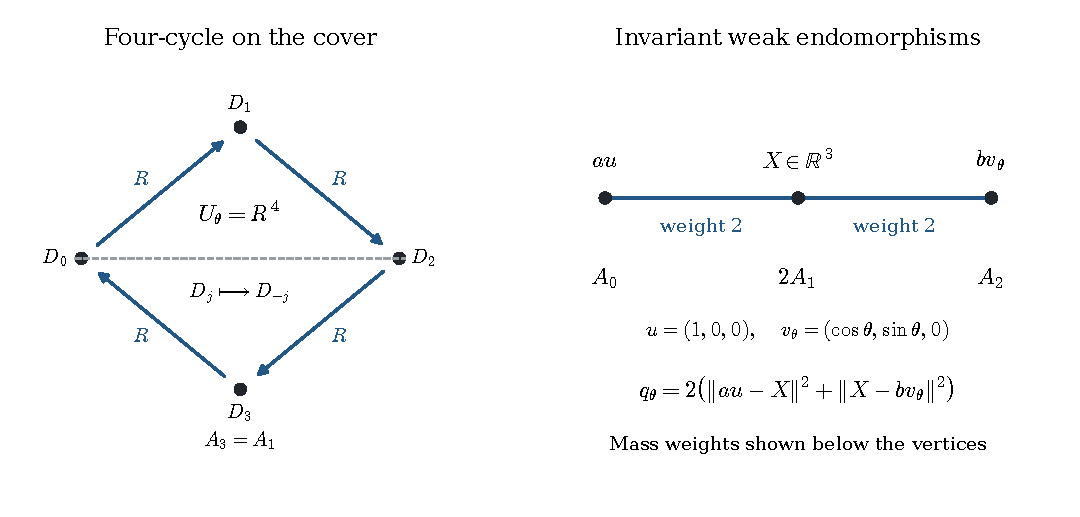
\includegraphics[width=\textwidth]{figures/output/gluing-constraints.pdf}
\caption{The four-cycle on the elliptic cover and its invariant
endomorphism problem. After an orthogonal change of middle frame,
the endpoint lines are $\RR u$ and $\RR v_\theta$.
The two edge coefficients are $2$, and the mass weights are
$A_0,2A_1,A_2$. The diagram represents the exact effective forms
\eqref{eq:five-forms}, not a numerical approximation of the HYM flow.}
\label{fig:gluing-constraints}
\end{figure}

\subsection{Equivariant capacity and mass estimates}
We record the curve estimates needed for the restriction to invariant
sections. Their constants concern the fixed elliptic family and a finite
number of component frames, and are uniform in the unitary transitions.
For a fixed small cutoff radius $a$, take paired node discs and invariant
component exteriors. A section with vertex values $X_j$ is extended by
affine interpolation in $\log|u|$ across a node annulus.
Conformal invariance of two-dimensional Dirichlet energy gives
\begin{equation}\label{eq:curve-trial}
 E(J_tX)=\frac{2\pi}{L+2\log a}\,q(X),\qquad
 \bigl|\|J_tX\|^2-m_A(X)\bigr|
       \le(Ca^2+o_a(1))m_A(X).
\end{equation}
Here $E(f)=\int_{E_t}|D_Vf|^2\,dA$, and $o_a(1)$ tends to zero
as $t\to0$ for fixed $a$. The mass error follows from convergence on
the component exteriors and the node-area bound $O(a^2)$.

Both trial interpolation and component averaging commute with the
involution. At a reflected node the logarithmic coordinate reverses,
and the two endpoints are transported by the verified unitary lift.
On a fixed component, averaging commutes with its isometry and the
constant frame map $J$. Consequently \eqref{eq:curve-trial} restricts
to the five-dimensional space \eqref{eq:linear-invariance}.

For a section $f$, let $b_j(f)$ be its mean on a fixed truncated
component. Poincar\'e and trace inequalities on that fixed component
bound the difference between $b_j(f)$ and the circular mean at an
incident boundary by $C_aE(f)^{1/2}$. Angular averaging and radial
Cauchy--Schwarz on the annulus then give
\begin{equation}\label{eq:curve-lower}
 q(b(f))^{1/2}
 \le\left(\sqrt{\frac{L+2\log a}{2\pi}}+C_a\right)E(f)^{1/2}.
\end{equation}
This is an estimate by the section's own energy, not an additive error
which could dominate a small positive eigenvalue.

For completeness, the mass estimate excluding extra weak modes is
\begin{equation}\label{eq:curve-mass}
 \bigl|m_A(b(f))-\|f\|^2\bigr|
 \le(Ca^2+C_a\sqrt\Lambda+o_a(1))\|f\|^2
\end{equation}
on a span of at most six eigensections with eigenvalues at most
$\Lambda\le1$. On fixed component collars, Poincar\'e and interior
elliptic estimates bound the boundary oscillation around the component
mean by $C_a\sqrt\Lambda$ for an orthonormal eigensection. Their
constants are uniform because the local flat equation and metric have
uniform fixed-chart bounds. The corresponding statement for a combination
of at most six eigensections follows by Cauchy--Schwarz.

On each annulus let $v$ be the harmonic section with the same boundary
values as $f$. The maximum principle controls $v$ by those boundary
values, and its mass is $O(a^2)$ times their squared bound.
The difference $f-v$ has zero boundary values and satisfies
\[
 \int_{\text{annulus}}|f-v|^2\,dA
       \le Ca^2\int_{\text{annulus}}|D_V(f-v)|^2\,dA
       \le Ca^2E(f).
\]
To obtain the first inequality uniformly in the annulus modulus,
use $F=|u|^2+|v|^2$ on the Euclidean curve $uv=t$.
Its divergence Laplacian is four and $|\nabla F|\le Ca$.
Integration by parts against the squared norm of a zero-boundary
section and Cauchy--Schwarz prove the inequality. The actual induced
metric is uniformly comparable to this metric, and Dirichlet energy
is conformally invariant. The second inequality follows from the
Dirichlet orthogonality of $v$ and $f-v$. Summing these bounds with
the component mass estimate proves \eqref{eq:curve-mass}. Invariant
sections have invariant means, so this estimate also restricts to
the required sector.

\begin{proof}[Proof of Theorem~\ref{thm:five-spectrum}]
The invariant trial map and min--max give five eigenvalues of order
$O(L^{-1})$ and their relative upper bounds. If a sixth invariant
curve eigenvalue tended to zero, choose $a$ small and then $t$ small.
Equation~\eqref{eq:curve-mass} would make the averaging map injective
from a six-dimensional spectral space into the five-dimensional
invariant tuple space, a contradiction. The invariant curve complement
therefore has a uniform positive gap $\gamma_E$.

Apply \eqref{eq:curve-lower} and \eqref{eq:curve-mass} on each initial
low spectral subspace and use finite-dimensional min--max. Along with
\eqref{eq:curve-trial}, they give the relative lower and upper bounds.
First fix $a$ for a prescribed error and then take $t$ small. This
produces one function $\varepsilon(t)\to0$ uniform in $\theta$;
no small effective eigenvalue is divided out in any estimate.

The product decomposition and \eqref{eq:norm-cancellation} transfer
these five eigenvalues to the threefold with the same coefficient.
Every other mode has lower bound
$\gamma=\min\{\gamma_S,\gamma_E\}$ after reducing it if necessary.
Finally zero energy means a compatible parallel tuple. In
\eqref{eq:five-forms} this is the equation $X=au=bv_\theta$,
which has one-dimensional solution space when $\sin\theta=0$ and
only the zero solution otherwise. It agrees with
\eqref{eq:parallel-algebra}, proving the exact kernel assertion.
\end{proof}

\begin{corollary}\label{cor:complement}
Let $\Pi_{t,\theta}$ be the orthogonal projection onto the five weak
eigenspaces, counting their exact kernel. On its orthogonal complement,
\[
 \|\mathcal L_{t,\theta}^{-1}(I-\Pi_{t,\theta})\|_{L^2\to L^2}
 \le\gamma^{-1},\qquad
 \|e^{-s\mathcal L_{t,\theta}}(I-\Pi_{t,\theta})\|_{L^2\to L^2}
 \le e^{-\gamma s}.
\]
For $z\notin[\gamma,\infty)$, the complementary resolvent has norm
at most $\operatorname{dist}(z,[\gamma,\infty))^{-1}$.
\end{corollary}

\begin{proof}
Apply the spectral theorem to the nonnegative self-adjoint operator
on the complementary subspace.
\end{proof}

These are $L^2$ estimates in the actual bundle metric. They do not
assert uniform global Schauder bounds across the degenerating necks.

\section{The constrained finite-dimensional metric evolution}\label{sec:finite-flow}

Let $\cP_r=\{H=H^*>0:\det H=1\}$. We use its affine invariant metric
and distance
\begin{equation}\label{eq:matrix-metric}
 g_H(V,W)=\tr(H^{-1}VH^{-1}W),\qquad
 d_r(H,K)^2=\tr\!\left(\log(H^{-1/2}KH^{-1/2})^2\right).
\end{equation}
Its geodesic is
\[
 \Geo(H,K;u)=H^{1/2}(H^{-1/2}KH^{-1/2})^uH^{1/2}.
\]
This is a complete simply connected space of nonpositive curvature;
the distance, geodesic and exponential metric inequality are reviewed
in \cite[Section 2.3]{bhatia}.
Congruence by an invertible matrix preserves its metric whenever the
congruence preserves the determinant-one locus. In particular unitary
transport is an isometry. Logarithms such as $\log(H^{-1}K)$ are
self-adjoint in the $H$ metric; they need not be Hermitian in the
identity frame.

The configuration space dictated by the bundle lift is
\begin{equation}\label{eq:finite-space}
 \cF=\{(H_0,H_1,H_2,H_3)\in\cP_2^4:
                   H_{-j}=JH_jJ^*\}.
\end{equation}
It is the fixed set of an isometric involution of the product with metric
$\sum_jA_jg_{H_j}$. It is therefore totally geodesic and geodesically
convex. More explicitly it is
$\cP_2^J\times\cP_2\times\cP_2^J$, with middle weight $2A_1$.
Each endpoint factor consists of $\exp(ae_x)$, $a\in\RR$, so
$\dim_\RR\cF=5$. The set is independent of $\theta$ in these frames;
the energy contains the parameter.

Put
\begin{equation}\label{eq:finite-potential}
 \Phi_{t,\theta}(H)=\frac\pi L\sum_{j\bmod4}
                d_2(H_{j+1},RH_jR^*)^2.
\end{equation}
Every edge appears once. The relation $JR=R^{-1}J$ makes this function
invariant under the involution defining \eqref{eq:finite-space}.

\begin{proposition}\label{prop:finite-flow}
The negative gradient flow of \eqref{eq:finite-potential} on $\cF$ is
the restriction of the four-vertex system
\begin{equation}\label{eq:finite-flow}
 A_jH_j^{-1}\dot H_j=\frac{2\pi}{L}
 \left\{\log(H_j^{-1}RH_{j-1}R^*)
             +\log(H_j^{-1}R^*H_{j+1}R)\right\}.
\end{equation}
For initial tuples in a fixed bounded set, it has a solution for every
physical time $s\ge0$, confined to a compact set independent of $t$ and
$\theta$. Distances between two solutions with the same parameters are
nonincreasing. The speed is $O(L^{-1})$, uniformly for all $s\ge0$;
the same bound holds for the time derivative of any fixed smooth tuple
function on the confined range.
\end{proposition}

\begin{proof}
The negative gradient in the first variable of
$\tfrac12d_2(H,K)^2$ is $H\log(H^{-1}K)$. Differentiating the two
incident terms and dividing by $A_j$ gives \eqref{eq:finite-flow}.
An invariant function has tangent gradient on the fixed set of an
isometric involution, so \eqref{eq:finite-space} is preserved. The
displayed logarithms are trace-free; the determinant condition is preserved.

Squared distance is jointly geodesically convex in this nonpositively
curved matrix space. Hence $\Phi$ is convex, and the identity tuple $I$
is a minimizer. The first-variation inequality for a convex function
gives
\[
 \frac{d}{ds}\frac12d_M(H(s),I)^2\le-\Phi(H(s))\le0,
\]
where $d_M^2=\sum_jA_jd_2^2$ is the product squared distance.
Closed bounded sets are compact in this finite-dimensional space,
proving confinement and continuation for all time. Applying the same
convexity inequality to the two geodesics between two solutions gives
nonexpansion. On the confined range every logarithm in
\eqref{eq:finite-flow} is bounded uniformly in the unitary $R$.
The equation then gives the speed and derivative bounds.
\end{proof}

The system is genuinely noncommuting. For example, choose $ab\ne0$ and
\[
 H_0=e^{a\sigma_x},\qquad H_1=e^{b\sigma_z},\qquad
 H_2=I,\qquad H_3=Je^{b\sigma_z}J^*=e^{-b\sigma_z}.
\]
This lies in $\cF$. In the common frame of the first edge,
$H_0$ and $R^*H_1R=H_1$ do not commute. Simultaneous frame conjugation
cannot remove this commutator, so the construction is not restricted
to independent scalar equations.

\begin{lemma}\label{lem:finite-decay}
Set $Z_j=\log H_j$,
$R_f=\tfrac12\sum_jA_j\|Z_j\|_{\HS}^2$, and
$\nu_0=(2\pi/L)\mu_0(\theta)$. Along \eqref{eq:finite-flow},
\begin{equation}\label{eq:finite-decay}
 \Phi(H)\ge\nu_0R_f,\qquad
 R_f'\le-2\Phi(H)\le-2\nu_0R_f.
\end{equation}
The linearization at the identity is the negative of the effective
operator with energy $(2\pi/L)q_\theta$ and mass $m_A$.
\end{lemma}

\begin{proof}
The logarithm based at the identity does not increase distance, so
\[
 d_2(H_{j+1},RH_jR^*)^2
       \ge\|Z_{j+1}-\Ad(R)Z_j\|^2.
\]
The logarithmic tuple satisfies \eqref{eq:linear-invariance}.
Using \eqref{eq:five-forms} gives the first inequality.

Radial contraction $H_j\mapsto e^{uZ_j}$ stays in $\cF$ and satisfies
$\Phi(e^{uZ})\le u^2\Phi(H)$ for $0\le u\le1$. This is the
distance contraction toward the common fixed point $I$. Differentiation
from the left at $u=1$ gives a radial derivative at least $2\Phi(H)$.
Pairing the negative gradient with the gradient of $R_f$ proves
\eqref{eq:finite-decay}. Finally expansion of the logarithms in
\eqref{eq:finite-flow} at $I$ gives the transported connection-graph
operator, whose restriction was computed in Section~\ref{sec:spectrum}.
\end{proof}

The parameter $\nu_0$ includes the exact zero mode at reducibility.
Thus \eqref{eq:finite-decay} gives a uniform exponential tail in $s/L$
on classes $\mu_0(\theta)\ge\kappa>0$. It does not give such a tail
when $\mu_0\to0$, although confinement and nonexpansion remain uniform.

\section{Reconstruction and the actual HYM flow}\label{sec:actual-flow}

On the actual rank-four bundle we use physical time $s$ and the equation
\begin{equation}\label{eq:hym-flow}
 h^{-1}\partial_sh=-2i\Lambda_{\omega_t}F_h.
\end{equation}
The Einstein constant is zero. All base and bundle parameters are fixed
in this equation. Relative to $h_0$, all metrics under consideration
have determinant one. For two rank-$r$ metrics put
\begin{equation}\label{eq:trace-distance}
 \sigma_r(h,k)=\tr(h^{-1}k+k^{-1}h)-2r.
\end{equation}
This expression is intrinsic, nonnegative, and at least $d_r(h,k)^2$.
On a fixed positive metric range it is uniformly equivalent to that
squared distance. For an approximate metric $k$, write
\[
 \mathcal R(k)=k^{-1}\partial_sk+2i\Lambda_{\omega_t}F_k.
\]

\begin{theorem}\label{thm:actual-tracking}
For each effective trajectory of \eqref{eq:finite-flow} with initial tuple
in a fixed bounded set, and all sufficiently small $t$, there is a smooth
determinant-one comparison metric $\widehat K(s)$ on $\cB_{t,\theta}$,
defined for every $s\ge0$, with uniform positive bounds against $h_0$,
such that
\begin{equation}\label{eq:global-residual}
 \sup_{s\ge0}\int_{X_t}|\mathcal R(\widehat K(s))|_{\op}\,dV_t
        \le C\frac{(1+\log L)^2}{L^2}.
\end{equation}
Let $h(s)$ solve \eqref{eq:hym-flow} from any smooth determinant-one
metric with $ch_0\le h(0)\le Ch_0$, for fixed positive bounds.
Set $\eta=\int_{X_t}\sigma_4(h(0),\widehat K(0))\,dV_t$ and
$e_L=(1+\log L)^2/L$. Then, for every $T\ge0$,
\begin{equation}\label{eq:bounded-tracking}
 \sup_{0\le s\le TL}\int_{X_t}d_4(h(s),\widehat K(s))^2\,dV_t
          \le\eta+CTe_L.
\end{equation}
The constants are independent of $\theta$, $t$, $s$ and $T$ in their
stated domains. The exact initial metric need not be a tensor metric.
\end{theorem}

\subsection{Equivariant reconstruction on the elliptic family}
The reconstruction uses a component correction cancelling the leading
velocity, flat geodesic interpolation on the necks, and an estimate
for their mismatch on the collars. We then tensor with the fixed
K3 metric and descend, keeping the full contracted Chern equation.
Put $\epsilon=L^{-1}$ and choose mean-zero component Green functions
\begin{equation}\label{eq:greens}
 \Delta_jg_{je}=-2\pi\delta_{p_{je}}+\frac{2\pi}{A_j},\qquad
 g_{je}=\log|u|+\gamma_{je}(u),
\end{equation}
where $\Delta_j$ is the nonnegative scalar Laplacian on $D_j$ and
$u$ is its node coordinate. Uniqueness makes these functions equivariant
under the isometry $\sigma$. The two actual incoming transports to
component $j$ are $U_{j,j-1}=R$ and $U_{j,j+1}=R^*$.
Define
\begin{equation}\label{eq:component-correction}
 B_{je}=\log(H_j^{-1}U_{jk}H_kU_{jk}^*),\qquad
 \xi_j=-\sum_{e\ni j}B_{je}g_{je},\qquad K_j=H_j e^{\epsilon\xi_j}.
\end{equation}
The logarithms are $H_j$-self-adjoint and trace-free. On the punctured
component, the effective equation gives the exact cancellation
\begin{equation}\label{eq:component-cancellation}
 \epsilon\Delta_j\xi_j=-H_j^{-1}\dot H_j.
\end{equation}

Cut at radius $\rho=L^{-1}$. At incidence $je$ write
\[
 \xi_j=-B_{je}\log|u|+c_{je}+q_{je}(u),\qquad q_{je}(0)=0.
\]
The corrected endpoint is $P_{je}=H_je^{\epsilon c_{je}}$.
On the node $j,k$, in the $j$ incidence frame, use
\begin{equation}\label{eq:node-geodesic}
 N_e(u)=\Geo(P_{je},U_{jk}P_{ke}U_{jk}^*;-\epsilon\log|u|).
\end{equation}
Reversing the geodesic and using $uv=t$ gives the same metric in the
other incidence frame. For each fixed time this node metric has zero
Chern curvature: if $P,Q$ are fixed endpoints, it is
$P\exp(-\epsilon\log|u|\log(P^{-1}Q))$, whose logarithmic derivative
has zero $\bar\partial$ away from the puncture.

Interpolate relative logarithms between $K_j$ and $N_e$ on
$\rho<|u|<2\rho$. Choose paired cutoffs, component transfers and node
charts under the involution. On fixed components the required smooth
transfer maps can be obtained from invariant lifts of base vector fields.
No holomorphic product trivialization is assumed. The operations
in \eqref{eq:component-correction}--\eqref{eq:node-geodesic} commute
with unitary transport, geodesic reversal and the actual lift
\eqref{eq:projective-lift}. Thus the resulting curve metric $K_E(s)$
is invariant in component \emph{and} node frames.

We give the residual estimate for this full Chern construction.
In a flat holomorphic frame, with
$\omega_{E_t}=(i/2)a\,dz\wedge d\bar z$, the actual equation is
\begin{equation}\label{eq:curve-chern-flow}
 \partial_sH=4a^{-1}(H_{z\bar z}-H_{\bar z}H^{-1}H_z).
\end{equation}
In real coordinates it contains
$i(H_xH^{-1}H_y-H_yH^{-1}H_x)$ as well as the two symmetric quadratic
terms. This commutator is retained in all curvature estimates below.

Effective-flow confinement and speed give, uniformly for all $s\ge0$,
\begin{equation}\label{eq:green-bounds}
 \begin{gathered}
 |B_{je}|\le C,\qquad |\dot B_{je}|\le C\epsilon,\qquad
 \|\xi\|_\infty\le C(1+|\log\rho|),\\
 \int\bigl(|\xi|+\epsilon^{-1}|\dot\xi|+|\nabla\xi|\bigr)\le C,
 \qquad \int|\nabla\xi|^2\le C(1+|\log\rho|).
 \end{gathered}
\end{equation}
These integrals are over the truncated components with their fixed metrics.
The identity
\[
 e^{-h}\partial e^h=\int_0^1e^{-uh}(\partial h)e^{uh}\,du
\]
and its differentiated form show that the component residual, after
\eqref{eq:component-cancellation}, is bounded by the integrals of
\[
 C\epsilon^2\bigl(|\xi|+|\xi|\,|\Delta_j\xi|
                                 +|\nabla\xi|^2\bigr).
\]
The second derivative is contracted before taking its norm: in complex
dimension one the $\bar\partial\partial\xi$ term in each conjugation
is a scalar multiple of $\Delta_j\xi$. Differentiating the conjugating
factors gives the displayed quadratic-gradient terms. Since
$\Delta_j\xi$ on the punctured component is bounded, the residual is
$O(\epsilon^2(1+|\log\rho|))$ after integration.
The time derivative of the correction has the same bound by
\eqref{eq:green-bounds} and $H_j^{-1}\dot H_j=O(\epsilon)$.

Here is the collar estimate which allows matching without losing this
order. For small endpoint logarithms $C_j,C_k$, let $D(C_j,C_k;u)$
be the relative logarithm at $H_j$ of
$\Geo(H_je^{C_j},U_{jk}H_ke^{C_k}U_{jk}^*;u)$, minus
$C_j+uB_{je}$. On the confined matrix range it is smooth, and
\[
 D(0,0;u)=0,\qquad D(C_j,C_k;0)=0.
\]
Bounded mixed derivatives imply
$|D|\le C(|C_j|+|C_k|)|u|$ and
$|\partial_uD|+|\partial_u^2D|\le C(|C_j|+|C_k|)$.
Substitute $C_j=\epsilon c_{je}$, $C_k=\epsilon c_{ke}$ and
$u=-\epsilon\log|z|$. Including the regular part $q_{je}$ gives
the mismatch bound, through two spatial derivatives,
\begin{equation}\label{eq:collar-mismatch}
 C\bigl(\epsilon\rho^{1-k}
             +\epsilon^2(1+|\log\rho|)\rho^{-k}\bigr),
 \qquad k=0,1,2.
\end{equation}
In the second derivative the additional term of order
$\epsilon^3\rho^{-2}$ is absorbed by the displayed bound.

The curvature difference from the exactly flat node profile contains
the second derivative of this mismatch, its first derivative times the
node logarithmic derivative $O(\epsilon/\rho)$, and its zeroth
derivative times the corresponding second-derivative and quadratic
terms. Cutoff derivatives have the same orders in $\rho$.
Since the collar area is $O(\rho^2)$, its integrated residual is
\[
 C\bigl(\epsilon\rho+
                 \epsilon^2(1+|\log\rho|)^2\bigr).
\]
The middle-node time residual is $O(\epsilon\rho^2)$; its spatial
Chern curvature is zero. Transfer to the actual smooth fibre adds
$C|t|\rho^{-N}$ for a fixed finite $N$, by the smooth plumbing
metric coefficients and the two derivatives in the contracted equation.
Putting $\rho=L^{-1}$ proves
\begin{equation}\label{eq:curve-residual}
 \sup_{s\ge0}\int_{E_t}
 |K_E^{-1}\dot K_E+2i\Lambda_{E_t}F_{K_E}|_{\op}\,dA
       \le C\frac{(1+\log L)^2}{L^2}.
\end{equation}
Every time-dependent input was a confined tuple or its
$O(L^{-1})$ velocity. Thus this is a residual bound on the whole
physical half-line, including reducible parameters.

\subsection{Exact tensor curvature and descent}
On the cover set $\widetilde K=h_S\otimes K_E$. Product Chern
connections give exact identities
\begin{equation}\label{eq:product-curvature}
 \begin{split}
 D_{\widetilde K}&=D_S\otimes I+I\otimes D_{K_E},\\
 F_{\widetilde K}&=F_{T^{1,0}S}\otimes I+I\otimes F_{K_E},\\
 \mathcal R(\widetilde K)&=I_{T^{1,0}S}\otimes
       (K_E^{-1}\dot K_E+2i\Lambda_{E_t}F_{K_E}).
 \end{split}
\end{equation}
The last equality uses the zero mean curvature of $h_S$. Equivariance
proved above makes $\widetilde K$ descend to $\widehat K$.
Its determinant is one in the fixed trivialization.
The operator norm of the tensor residual is unchanged, whereas
integration divides by the degree two of the cover. Consequently
\eqref{eq:curve-residual} implies \eqref{eq:global-residual}.

For two tensor metrics there is also the exact distance identity
\begin{equation}\label{eq:tensor-distance}
 d_4(h_S\otimes H,h_S\otimes K)^2=2d_2(H,K)^2.
\end{equation}
Together with \eqref{eq:k3-volume}, division by the cover degree
makes their global quotient squared distance equal to the curve
integral. Neither tensor identity is assumed for an arbitrary exact
solution $h(s)$.

\subsection{Intrinsic comparison for arbitrary rank-four metrics}
On each fixed compact smooth fibre, the classical HYM metric flow
exists for all time; see \cite[Section 4.1, after (4.8)]{hkkp}.
Order comparison \cite[Proposition 4.3]{hkkp}
with $ch_0$ and $Ch_0$ preserves
the bounds, and the scalar determinant equation preserves the
normalization. These fixed-fibre statements impose no uniform
Sobolev-constant hypothesis on the degenerating family.

For an exact flow $h$ and a comparison metric $k$ in a common fixed
positive range, the Chern trace calculation gives
\begin{equation}\label{eq:forced-trace}
 (\partial_s+\Delta_{\omega_t})\sigma_4(h,k)
                \le C|\mathcal R(k)|_{\op}.
\end{equation}
For two exact velocities, the intrinsic trace calculation of
\cite[Proposition 2.4]{wang}, with the coupling section set to zero,
makes the left side a sum of nonpositive
quadratic derivative terms in local holomorphic frames. Replacing the
velocity of $k$ by its exact-flow velocity plus $k\mathcal R(k)$
adds the traces of $h^{-1}k\mathcal R(k)$ and its inverse-metric
counterpart. Their absolute values are bounded by the right side
under the fixed relative bounds. The same calculation is summed over
all complex coordinate directions. It is intrinsic and therefore
applies across the nonflat tangent-bundle frames, without reducing
the exact solution to a tensor ansatz.

\begin{proof}[Proof of Theorem~\ref{thm:actual-tracking}]
The equivariant construction and \eqref{eq:product-curvature} prove
the comparison metric and its residual estimate. Integrate
\eqref{eq:forced-trace} on the closed smooth fibre, so that the
Laplacian integrates to zero. Its accumulated right side up to time
$TL$ is at most $CT(1+\log L)^2/L$. Since $d_4^2\le\sigma_4$,
this proves \eqref{eq:bounded-tracking}. No derivative bound on
the exact initial metric enters this argument.
\end{proof}

\begin{theorem}\label{thm:all-time}
Under the hypotheses of Theorem~\ref{thm:actual-tracking}, assume also
$\mu_0(\theta)\ge\kappa>0$. For sufficiently small $t$,
\begin{equation}\label{eq:all-time}
 \sup_{s\ge0}\int_{X_t}d_4(h(s),\widehat K(s))^2\,dV_t
       \le C\eta+C_\kappa e_L(1+|\log e_L|).
\end{equation}
\end{theorem}

\begin{proof}
For the actual flow write $h=h_0H=h_0e^{\Psi}$. Pointwise $\tr \Psi=0$.
The exact relative Chern equation is
\[
 H_s=-D_\theta^*D_\theta H
       -4\sum_\alpha(D_\alpha H)^*H^{-1}(D_\alpha H).
\]
The contracted background-curvature commutator is zero. All quadratic
terms are retained, including those from noncommuting derivatives.
Put $F(s)=\int_{X_t}\tr(e^{\Psi}-I)\,dV_t$. On the fixed positive range,
Taylor's formula and trace freeness give
\[
 \frac c2\|\Psi\|_{L^2}^2\le F\le\frac C2\|\Psi\|_{L^2}^2,
 \qquad -F'\ge\frac{c^2}{C}\int_{X_t}|D_\theta \Psi|^2\,dV_t.
\]
For the derivative inequality first bound $H^{-1}\ge C^{-1}I$
inside the positive quadratic term. The unweighted trace then satisfies
$4\sum_\alpha\tr((D_\alpha H)^*D_\alpha H)=|D_\theta H|^2$.
The divided differences of the exponential on the bounded spectrum
are at least $c$, giving $|D_\theta H|\ge c|D_\theta \Psi|$.
No commutator is discarded inside a matrix-weighted trace.

There is no trace-free parallel kernel on the stated parameter class.
Theorem~\ref{thm:five-spectrum} therefore gives
\[
 F(s)\le F(0)\exp\left(
 -\frac{2c^2}{C^2}(1-\varepsilon(t))\frac{2\pi\mu_0(\theta)}{L}s
 \right).
\]
Lemma~\ref{lem:finite-decay} gives a corresponding exponential tail
for the effective trajectory. The reconstruction is uniformly Lipschitz
in global $L^2$ on the confined tuple range: the Green coefficients
have bounded $L^2$ norms multiplied by $L^{-1}$, and the node and
collar maps have bounded tuple derivatives. It sends the identity tuple
exactly to $h_0$. Equation~\eqref{eq:tensor-distance} therefore
transfers effective-flow decay to the comparison metric.

For $s\ge TL$, the exact and reconstructed squared distances to
$h_0$ are at most $C e^{-c_\kappa T}$. For $s\le TL$, use
\eqref{eq:bounded-tracking}. Taking $T$ proportional to
$1+|\log e_L|$ and applying the squared triangle inequality proves
\eqref{eq:all-time}.
\end{proof}

The all-time conclusion is uniform on a nonempty stable parameter class.
At reducibility there are nonidentity parallel metrics, and as
$\mu_0\to0$ the above tail constants degenerate. The bounded-time
comparison remains uniform there; extending it to the weakest inverse
rate requires a further argument.

\section{Phase selection on a fixed Hermitian--Einstein bundle}
\label{sec:parallel-phase}

The component metrics required for spatial initial data are selected by
an intrinsic fixed-background argument. Let $(Y,\omega)$ be a connected
compact K\"ahler manifold of volume $V$. Let $(E,h_0)$ be a
Hermitian--Einstein bundle of rank $r$, with Chern connection $D$ and
$i\Lambda F_D=\lambda I$. Write $h=h_0H$ and use the normalized equation
\begin{equation}\label{eq:fixed-flow}
 H^{-1}H_s=-2(i\Lambda F_h-\lambda I),\qquad \det H=1.
\end{equation}
The base and connection are fixed throughout this section. The positive
gap used here is not asserted to be uniform on a degenerating family.

Let $\mathcal A$ be the algebra of $D$-parallel complex endomorphisms,
and let $\Pi$ be the $L^2$ orthogonal projection onto $\mathcal A$.
Denote by $\lambda_\perp>0$ the first positive eigenvalue of $D^*D$
on self-adjoint endomorphisms, with its parallel kernel omitted.

\begin{theorem}\label{thm:parallel-phase}
Suppose $H(0)$ is smooth, $\det H(0)=1$ and $cI\le H(0)\le CI$,
where $0<c\le C<\infty$. There is a unique positive parallel
endomorphism $P=P(H(0))$, with $\det P=1$, to which $H(s)$ converges
in $L^2$ and uniformly. Put
\begin{equation}\label{eq:phase-functionals}
 M=\Pi H,\qquad \mathcal J=\log\det M,\qquad
 W=V^{-1}\int_Y|H-M|^2\,dV,\qquad
 \gamma=\frac{2c^2\lambda_\perp}{C^2}.
\end{equation}
Then $M$ decreases in matrix order to $P$, and
\begin{equation}\label{eq:phase-estimates}
 \frac{W}{2C^2}\le \mathcal J\le\frac{W}{2c^2},\qquad
 \mathcal J(s)\le \mathcal J(0)e^{-\gamma s},\qquad
 \tr(M(s)-P)\le C\mathcal J(s).
\end{equation}
In particular,
\begin{equation}\label{eq:phase-l2}
 V^{-1}\int_Y|H(s)-P|^2\,dV
       \le C^2(2\mathcal J(0)+\mathcal J(0)^2)e^{-\gamma s}.
\end{equation}
For $s\ge1$ the squared affine distance satisfies
\begin{equation}\label{eq:phase-uniform}
 \sup_Y d_r(H(s),P)^2
       \le K_Y(2\mathcal J(0)+\mathcal J(0)^2)e^{-\gamma(s-1)}.
\end{equation}
Here $K_Y$ also depends on $c,C,r$ and the fixed background. For two
initial metrics in a common positive range, the selected phases obey
\begin{equation}\label{eq:phase-contraction}
 V\sigma_r(P(H(0)),P(K(0)))
       \le\int_Y\sigma_r(H(0),K(0))\,dV.
\end{equation}
Consequently phase selection is Lipschitz on such a range. If
$\mathcal A=\CC I$, the selected phase is $I$.
\end{theorem}

\begin{proof}
Decompose the unitary holonomy representation at a base point into
inequivalent irreducible representations and their multiplicity spaces.
Parallel transport of the invariant summands gives a global orthogonal
parallel decomposition
\begin{equation}\label{eq:holonomy-splitting}
 E=\bigoplus_a F_a\otimes\CC^{m_a},\qquad
 D=\bigoplus_a D_a\otimes I,
 \qquad \mathcal A=\bigoplus_a I_{F_a}\otimes\End(\CC^{m_a}).
\end{equation}
The transported subspaces are independent of the chosen path because
they are holonomy invariant. This does not require individual parallel
vectors on $F_a$. The splitting is also holomorphic since the
$(0,1)$ part of $D$ is the holomorphic structure.

If $r_a=\operatorname{rank}F_a$ and $B_{aa}$ is a diagonal block of
an endomorphism section, direct testing against every parallel
endomorphism gives
\begin{equation}\label{eq:parallel-projection}
 \Pi B=\bigoplus_a I_{F_a}\otimes
       \frac1{r_aV}\int_Y\tr_{F_a}B_{aa}\,dV.
\end{equation}
The partial trace is globally defined using the fixed metric on $F_a$.
Diagonal restriction, partial trace and integration preserve positivity.
Thus $\Pi$ is positive, unital and adjoint preserving. It preserves the
normalized integrated trace, and, for any parallel endomorphism $B$,
\begin{equation}\label{eq:projection-trace}
 \tr(B\Pi Q)=V^{-1}\int_Y\tr(BQ)\,dV.
\end{equation}
Order comparison for \eqref{eq:fixed-flow} preserves $cI\le H\le CI$;
its scalar determinant equation preserves $\det H=1$. Hence
$cI\le M\le CI$.

We need the full relative metric equation. In unitary normal base
coordinates with $\omega=(i/2)\sum dz_\alpha\wedge d\bar z_\alpha$
at the point, expansion of $\bar\partial_D(H^{-1}\partial_DH)$ gives
\begin{equation}\label{eq:relative-fixed-equation}
 H_s=-D^*DH-Q(H),\qquad
 Q(H)=4\sum_\alpha(D_\alpha H)^*H^{-1}(D_\alpha H)\succeq0.
\end{equation}
The second-order term has scalar principal part
$4\sum\partial_\alpha\partial_{\bar\alpha}H$. Its difference from
$-D^*DH$ on endomorphism-valued zero-forms is the contracted curvature
commutator, which vanishes because $i\Lambda F_D=\lambda I$.
Differentiating $H^{-1}$ gives precisely the displayed quadratic term.
In particular, it cannot be dropped for matrix-valued $H$.
Since $\Pi D^*DH=0$, positivity of the projection proves
\begin{equation}\label{eq:monotone-mean}
 M'=-\Pi Q(H)\preceq0.
\end{equation}
It follows that $M$ has a parallel positive limit $P$ between $cI$ and $CI$.

Taylor's integral remainder for $\log\det$ on the segment from $M$
to $H$ has Hessian between $-c^{-2}$ and $-C^{-2}$ in Frobenius norm.
The integrated linear term vanishes, since
\[
 V^{-1}\int_Y\tr(M^{-1}(H-M))\,dV=0
\]
by \eqref{eq:projection-trace}. Integrating $\log\det H=0$ gives
the two bounds for $\mathcal J$ in \eqref{eq:phase-estimates}.
Next, the same trace identity and positivity give
\begin{align*}
 -\mathcal J'&=V^{-1}\int_Y\tr(M^{-1}Q(H))\,dV\\
     &\ge C^{-2}V^{-1}\int_Y|DH|^2\,dV
      \ge C^{-2}\lambda_\perp W\ge\gamma \mathcal J.
\end{align*}
For the first inequality, remove both positive matrix weights using
their lower bounds. Only then use
$4\sum_\alpha\tr((D_\alpha H)^*D_\alpha H)=|DH|^2$.
The gap applies because $H-M$ is orthogonal to the whole parallel
algebra and $D(H-M)=DH$. This proves exponential decay of $\mathcal J$.

By continuity, $\log\det P=0$. Integrating the derivative of
$\log\det$ on the positive segment from $P$ to $M$ gives
$\tr(M-P)\le C\mathcal J$. Orthogonality to parallel sections gives the exact
decomposition
\[
 V^{-1}\int_Y|H-P|^2\,dV=W+|M-P|^2
       \le 2C^2\mathcal J+C^2\mathcal J^2.
\]
Here $M-P\succeq0$, so its norm is at most its trace. This proves
\eqref{eq:phase-l2}.

The metric $h_0P$ has the same Chern connection as $h_0$ and is
stationary. The unforced trace comparison from
\eqref{eq:forced-trace}, followed by the time-one scalar heat kernel
on the fixed compact base, bounds the supremum of
$\sigma_r(H(s),P)$ by a fixed multiple of its integral at $s-1$.
Equivalence of trace distance and squared norm on the fixed range
proves \eqref{eq:phase-uniform}. This uses no derivative bound on
arbitrary bounded initial metrics and no degenerating heat kernel.

Finally, integrate the trace comparison for two exact flows. Uniform
convergence to their parallel limits proves \eqref{eq:phase-contraction}.
It also gives uniqueness, and the equivalence of the distances gives
the stated Lipschitz dependence. A positive scalar endomorphism with
determinant one is the identity.
\end{proof}

On a bundle with repeated irreducible factors the phase belongs to the
actual algebra \eqref{eq:holonomy-splitting}; it is not a constant matrix
in a chosen local frame on the whole bundle. In the next section the
fixed component bundles supply this algebra and its positive gap.
The global degeneration estimate will be established separately.

\section{Entry from spatial initial metrics}\label{sec:spatial-entry}

The four fixed component problems on the cover have bases and bundles
\begin{equation}\label{eq:component-bundles}
 Y_j=S\times D_j,\qquad F_j=p_S^*T^{1,0}S\otimes\CC^2,
 \qquad h_{j,0}=h_S\otimes I.
\end{equation}
They have zero Einstein constant and complex parallel algebra
$I_{T^{1,0}S}\otimes\End(\CC^2)$. Their geometry is independent of
$t$ and $\theta$; the latter enters the node identifications. Thus
Theorem~\ref{thm:parallel-phase} selects, from each smooth
determinant-one component metric, a phase $I_{T^{1,0}S}\otimes P_j$.
Positivity and $(\det P_j)^2=1$ give $\det P_j=1$. For equivariant
initial profiles, uniqueness of the component flow gives
$P_{-j}=JP_jJ^*$. The selected tuple belongs to the finite-dimensional
configuration space of Section~\ref{sec:finite-flow}.

\subsection{The open class and its topology}
Put $\rho=L^{-1}$ and let $\Omega_j(2\rho)\subset D_j$ be the
complement of the two open node discs of radius $2\rho$. Use the
equivariant smooth component transfers already fixed in the
reconstruction. An actual initial metric on $\cB_{t,\theta}$ pulls
back to $h_0e^{\Psi_{\mathrm{in}}}$, where $\Psi_{\mathrm{in}}$ is a smooth
equivariant trace-free $h_0$-Hermitian endomorphism. Its restriction to
the $j$th component exterior is a section $\Psi_j$ on
$S\times\Omega_j(2\rho)$ with values in $\Herm_0(F_j)$.

Fix $0<\beta<1$ and $R_0>0$. Using the fixed component connections and
metrics in all component norms, define
\begin{equation}\label{eq:extension-norm}
 \begin{split}
 \mathcal N_t(\Psi)={}&\|\Psi\|_{C^0(X_t)}+
 \inf\left\{\sum_{j=0}^3\|\widetilde\Psi_j\|_{C^{6,\beta}(Y_j)}:
       \widetilde\Psi_j|_{S\times\Omega_j(2\rho)}=\Psi_j,\right.\\[-2pt]
 &\hspace{49mm}\left.(\widetilde\Psi_j)_{j=0}^3
                    \text{ is an equivariant smooth extension}\right\},\\
 \mathcal B_{R_0}(t,\theta)={}&
       \{h_0e^{\Psi}:\mathcal N_t(\Psi)<R_0\}.
 \end{split}
\end{equation}
Equivariance includes the base involution and the actual component
bundle lift $(i\,d\iota)\otimes J$, not just conjugation of a matrix.

\begin{lemma}\label{lem:open-class}
For every fixed smooth fibre, $\mathcal B_{R_0}(t,\theta)$ is a
nonempty open set in the $C^{6,\beta}$ topology on smooth
determinant-one metrics. It contains a parameter-independent small
ball of smooth equivariant component profiles, joined across the
nodes, and contains metrics which are not tensor products.
\end{lemma}
\begin{proof}
Each component exterior is a compact manifold with smooth boundary.
Smooth collar extension operators for its bundle sections are bounded
in the fixed $C^{6,\beta}$ norms. Averaging the operators over the
finite involution preserves equivariance, Hermitian symmetry and zero
trace. For a fixed fibre their operator bounds, together with the
triangle inequality for the infimum in \eqref{eq:extension-norm},
prove continuity of $\mathcal N_t$. The global $C^0$ term makes it
a norm, and exponentiation is smooth. No uniform extension-operator
bound as $\rho\to0$ is used. In particular the radius in
\eqref{eq:extension-norm} is not a radius for an unrestricted global
$C^0$ norm.

Take a sufficiently small fixed ball of equivariant smooth component
logarithms and join their metrics by fibrewise geodesics on the necks.
The original profiles are admissible extensions; compactness of the
positive matrix range bounds the interpolated logarithms. This yields
members of the asserted class for all small $t$. Smooth modifications
supported in the middle necks with sufficiently small $C^0$ amplitude
are allowed, independently of their derivatives.

For a non-tensor example, take a nonzero local section
$A(x)\in\Herm_0(T^{1,0}S)$ and a real smooth function $\chi(z)$
supported away from the nodes. Choose the support disjoint from its
deck image, possible because $\iota$ is free, and average the
transported logarithm $\chi(z)A(x)\otimes\sigma_z$ under the deck
action. Its mixed trace-free component remains nonzero on the original
support. Small multiples belong to the class. For positive $G,K$,
\[
 \log(G\otimes K)=(\log G)\otimes I+I\otimes(\log K),
\]
whose projection to
$\Herm_0(T^{1,0}S)\otimes\Herm_0(\CC^2)$ is zero. Uniqueness of
the Hermitian logarithm therefore excludes tensor factorization of
the example. These initial metrics can depend on all six real spatial
coordinates and need not commute with the tangent curvature.
\end{proof}

\subsection{Component evolution and the choice of phase}
Choose an equivariant extension tuple in \eqref{eq:extension-norm}
with total norm less than $2R_0$. Let $\Phi_j(s)$ be its relative
metric under the exact HYM flow on $Y_j$. Theorem~\ref{thm:parallel-phase}
and the fixed component gaps give constants depending only on $R_0$
and the fixed geometry such that
\begin{equation}\label{eq:component-phase-rate}
 \sup_{Y_j}d_4(\Phi_j(s),I\otimes P_j)^2
       \le C_{R_0}e^{-\gamma_{R_0}(s-1)},\qquad s\ge1.
\end{equation}
All these flows remain in a common compact positive range.
For every finite integer $n$, there is a common constant $C_n$
bounding their spatial covariant derivatives through order three and
their time derivatives on $0\le s\le n$. Indeed, the bounded
$C^{6,\beta}$ initial set is precompact in $C^{4,\beta/2}$ on the
fixed compact $Y_j$. The relative equation has scalar elliptic
principal part and a smooth quadratic-gradient nonlinearity on the
fixed positive range. Local parabolic continuous dependence,
smoothing and fixed-base global continuation give bounds on a
neighbourhood of each initial datum in the compact closure. A finite
cover gives $C_n$. Enlarge them to be nondecreasing and at least one.
This argument uses component derivative control, rather than drawing
derivative estimates from an arbitrary $C^0$ bound.

Two allowed extensions of the same initial metric differ only on
$S$ times discs of total area $O(\rho^2)$ and remain in a fixed
positive range. Their initial trace-distance integral is therefore
$O_{R_0}(\rho^2)$. The phase contraction
\eqref{eq:phase-contraction} implies
\begin{equation}\label{eq:phase-ambiguity}
 d_2(P_j,P'_j)^2\le C_{R_0}\rho^2.
\end{equation}
The factor two in the rank-four tensor distance and the fixed component
volume are included in the constant. Thus the phase is determined up
to $O(\rho)$, without claiming an exactly canonical extension at
finite $t$. Effective-flow nonexpansion preserves this bound at all times.

\begin{theorem}\label{thm:spatial-entry}
There is a preparation time $s_*(t)\to\infty$, with $s_*(t)/L\to0$,
independent of $\theta$ and of the initial metric in
$\mathcal B_{R_0}(t,\theta)$, with the following property.
Let $P$ be a component phase tuple selected as above. Let $H_f(s)$
solve the effective equation with $H_f(0)=P$, and let
$\widehat K(H_f(s))$ be its reconstruction. The actual HYM solution
from any metric in this open class satisfies
\begin{equation}\label{eq:entry-eta}
 \begin{gathered}
 \eta_*:=\int_{X_t}\sigma_4(h(s_*),\widehat K(P))\,dV_t
     \le C_{R_0}\left(\sqrt{\delta_L}
          +e^{-\gamma_{R_0}(s_*-1)}+L^{-2}\right)\longrightarrow0,\\
 \delta_L=\frac{1+\log L}{L}+|t|L^N,
 \end{gathered}
\end{equation}
where $N$ is a fixed finite exponent. For each $T\ge0$,
\begin{equation}\label{eq:spatial-bounded}
 \sup_{s_*\le s\le s_*+TL}\int_{X_t}
 d_4(h(s),\widehat K(H_f(s-s_*)))^2\,dV_t
       \le \eta_*+C_{R_0}Te_L.
\end{equation}
If also $\mu_0(\theta)\ge\kappa>0$, then
\begin{equation}\label{eq:spatial-alltime}
 \sup_{s\ge s_*}\int_{X_t}d_4(h(s),\widehat K(H_f(s)))^2\,dV_t
 \le C_{R_0}\eta_*+C_{R_0,\kappa}e_L(1+|\log e_L|)
                 +C_{R_0}(s_*/L)^2.
\end{equation}
All estimates before the last one are uniform through
$\theta\in\pi\ZZ$.
\end{theorem}

\begin{proof}
On the component exteriors transfer $\Phi_j(s,x,z)$ to the actual
smooth fibre. At incidence $je$ put
$A_{je}(s,x)=\Phi_j(s,x,p_{je})$. In a common node frame join the
two transported endpoints by the rank-four affine geodesic with
parameter $-L^{-1}\log|u|$. At the oriented node $j,j+1$, the
right endpoint is
\[
 (I\otimes R^*)A_{j+1,e}(I\otimes R),
\]
as follows from the actual incidence relation $w_{j+1}=Rz_j$.
Interpolate to the component metrics on $\rho<|u|<2\rho$ by
equivariant relative-logarithm cutoffs. All these constructions are
intrinsic in the positive metrics on $T^{1,0}S\otimes\CC^2$ and
respect the deck lift. They define a descended preparation metric
$K_{\mathrm{pre}}(s)$ in a fixed positive range. At $s=0$ it agrees
with the actual initial metric on the component exteriors.

We estimate its full contracted Chern residual for $0\le s\le n$.
On component regions the comparison solves the full rank-four
equation for the fixed product metric, including tangent curvature
and all spatially varying noncommuting terms. The only transfer
error is from the elliptic geometry. Smooth plumbing coefficients,
with the required two derivatives and the $C_n$ bounds, give integrated
error $C_n|t|\rho^{-N}$ for a fixed finite $N$ independent of $n$.

On a node interior, for each fixed $x\in S$ the geodesic has zero
Chern curvature in the curve direction. Its $S$-direction curvature
generally does not vanish. Covariant $S$ derivatives through order
two of the geodesic are bounded by $C_n$ on the compact endpoint
range. The tangent background has zero mean curvature, so the
$S$-contracted residual is $O(C_n)$. The time residual has the same
bound. Mixed $S$/curve curvature components can be nonzero but
contract to zero with the exact block diagonal product K\"ahler
form. Since the middle-node volume is $O(\rho^2)$, these terms
contribute $C_n\rho^2$ in integral. Thus the argument does not
assert vanishing of the full spatial curvature.

On an incidence collar the component endpoint discrepancy and the
geodesic discrepancy, with their first two curve derivatives, obey
\begin{equation}\label{eq:preparation-collar}
 C_n\bigl(\rho+L^{-1}|\log\rho|\bigr)\rho^{-k},
                    \qquad k=0,1,2.
\end{equation}
For the component term this is Taylor expansion in the curve coordinate;
for the geodesic term it is differentiation of the smooth endpoint
map at parameter $O(L^{-1}|\log\rho|)$. The relevant mixed
derivatives are included in $C_n$. Expanding the contracted Chern
expression relative to the node profile, the second derivatives of
the discrepancy and the cutoff terms integrate to
$C_n(\rho+L^{-1}|\log\rho|)$. Products with the node derivative
$O((L\rho)^{-1})$ satisfy the same bound, as do quadratic mismatch
terms for small $\rho+L^{-1}|\log\rho|$. This calculation is valid
for arbitrary rank-four matrices. The cutoff is independent of $S$,
so $S$ derivatives and time derivatives still contribute only
$C_n\rho^2$. Mixed contractions remain zero. Taking $\rho=L^{-1}$
therefore proves
\begin{equation}\label{eq:preparation-residual}
 \sup_{0\le s\le n}\int_{X_t}
       |\mathcal R(K_{\mathrm{pre}}(s))|_{\op}\,dV_t
                  \le C_n\delta_L.
\end{equation}

At time zero the exact and preparation metrics differ only in regions
of volume $O(\rho^2)$. Boundedness gives initial integrated trace
distance at most $C_{R_0}\rho^2$, regardless of the initial neck
derivatives. The forced trace comparison gives
\begin{equation}\label{eq:preparation-comparison}
 \sup_{0\le s\le n}\int_{X_t}
 d_4(h(s),K_{\mathrm{pre}}(s))^2\,dV_t
                \le C_{R_0}\rho^2+nC_n\delta_L.
\end{equation}
Choose
\begin{equation}\label{eq:preparation-time}
 s_*=\max\{n\in\mathbb N:nC_n\le\delta_L^{-1/2}\}.
\end{equation}
For small $t$ this set is nonempty and finite. Each fixed integer
eventually belongs to it, so $s_*\to\infty$. Moreover
$s_*C_{s_*}\delta_L\le\sqrt{\delta_L}$ and
$s_*/L\le\sqrt{\delta_L}$, using $C_n\ge1$ and $\delta_L\ge L^{-1}$.
This is an implicit common time; no logarithmic formula for it is claimed.

On the component exteriors at $s_*$, use
\eqref{eq:component-phase-rate}. The Green correction in
$\widehat K(P)$ has global $L^2$ size $O(L^{-1})$.
On the remaining node regions boundedness and volume $O(\rho^2)$
suffice. Therefore
\[
 \int_{X_t}d_4(K_{\mathrm{pre}}(s_*),\widehat K(P))^2\,dV_t
       \le C_{R_0}(e^{-\gamma_{R_0}(s_*-1)}+L^{-2}).
\]
Combine this with \eqref{eq:preparation-comparison} and the equivalence
of trace distance and squared affine distance on the fixed positive
range to obtain \eqref{eq:entry-eta}. Apply
Theorem~\ref{thm:actual-tracking} starting at $s_*$ to obtain
\eqref{eq:spatial-bounded}.

The effective speed is $O(L^{-1})$ for every time, so
$d_M(H_f(s-s_*),H_f(s))\le C_{R_0}s_*/L$ for $s\ge s_*$,
where $d_M$ is the mass-weighted product distance. The reconstruction
is uniformly Lipschitz into global $L^2$ on the confined tuple range.
Thus changing to the physical-time-aligned comparison costs at most
$C_{R_0}(s_*/L)^2$, with fixed squared-triangle constants. Under the
positive-rate hypothesis, Theorem~\ref{thm:all-time} applied after
entry proves \eqref{eq:spatial-alltime}.
\end{proof}

The extension ambiguity \eqref{eq:phase-ambiguity}, effective-flow nonexpansion
and the reconstruction bound show that changing the allowed component
extensions changes all subsequent comparisons by $O(L^{-1})$ in
$L^2$ distance. The theorem gives entry from a fixed-radius open class
with genuine spatial variation. It does not give trajectory tracking
during the preparation interval, uniform derivative estimates over
the whole neck, or an all-time bound as $\mu_0$ tends to zero.

\section{Transport recovery and the order of limits}\label{sec:inverse-limits}

\subsection{The observed invariant}
In this inverse problem the compact family and its unitary
one-parameter bundle class are known. The normalization
$L=\log(1/|t|)$ and the three component areas $A_0,A_1,A_2$ are known.
The parameter $\theta$, the transition matrices and their cycle
product are not supplied. The observations are the five lowest
eigenvalues of the actual operator $\mathcal L_{t,\theta}$, including
its zero modes. The target is the conjugacy class of
$\Ad(U_\theta)$ in $\operatorname{SO}(3)$.
It is a global bundle-transport invariant. The integral Chern number
computed in Section~\ref{sec:geometry} is not an output of this
spectral inverse.

\begin{theorem}\label{thm:transport-inverse}
With the above observations define
\begin{equation}\label{eq:transport-estimator}
 \widehat s_t=\frac{A_0A_1^3A_2}{8}
     \left(\frac{L}{2\pi}\right)^5\prod_{k=0}^4\lambda_k(t,\theta).
\end{equation}
For the error in Theorem~\ref{thm:five-spectrum},
\begin{equation}\label{eq:inverse-relative}
 (1-\varepsilon(t))^5\sin^2\theta
 \le\widehat s_t\le(1+\varepsilon(t))^5\sin^2\theta.
\end{equation}
Thus $3-4\widehat s_t$ recovers $\tr\Ad(U_\theta)$ with error
$O(\varepsilon(t)\sin^2\theta)$. If
$\operatorname{clip}(x)=\max(0,\min(1,x))$, then
\begin{equation}\label{eq:angle-estimator}
 \widehat\alpha_t=2\arcsin\sqrt{\operatorname{clip}(\widehat s_t)}
\end{equation}
converges uniformly over the family to its principal projective
conjugacy angle in $[0,\pi]$.
On a class $\sin^2\theta\in[\kappa,1-\kappa]$, $0<\kappa<1/2$,
the angle error is at most $C_{A,\kappa}(\varepsilon(t)+\delta)$
if each observed rescaled eigenvalue $L\lambda_k/(2\pi)$ has
additive error at most $\delta$, for small $\delta$ and $t$.
\end{theorem}

\begin{proof}
In coordinates $(a,x,y,z,b)$ write $c_\theta=\cos\theta$ and
$s_\theta=\sin\theta$. The energy and mass matrices are
\begin{equation}\label{eq:five-matrices}
 Q_\theta=\begin{pmatrix}
 2&-2&0&0&0\\
 -2&4&0&0&-2c_\theta\\
 0&0&4&0&-2s_\theta\\
 0&0&0&4&0\\
 0&-2c_\theta&-2s_\theta&0&2
 \end{pmatrix},\qquad
 M_A=\operatorname{diag}(A_0,2A_1,2A_1,2A_1,A_2).
\end{equation}
The Schur complement of the middle $4I_3$ block is
$\left(\begin{smallmatrix}1&-c_\theta\\-c_\theta&1\end{smallmatrix}\right)$.
Consequently
\begin{equation}\label{eq:determinant-product}
 \det Q_\theta=64\sin^2\theta,\qquad
 \prod_{k=0}^4\mu_k(\theta)
       =\frac{8\sin^2\theta}{A_0A_1^3A_2}.
\end{equation}
Multiplying the five relative bounds in
\eqref{eq:five-relative} proves \eqref{eq:inverse-relative}.
At $\theta\in\pi\ZZ$ both products are exactly zero.

Since $U_\theta=\operatorname{diag}(e^{i\theta},e^{-i\theta})$,
its adjoint rotation has trace
$1+2\cos(2\theta)=3-4\sin^2\theta$. The principal angle is
$2\arcsin\sqrt{\sin^2\theta}$. Uniform continuity on $[0,1]$
proves uniform recovery after clipping. On the stated interior class
the derivative of this function is bounded, which proves Lipschitz
dependence on the estimator.

The rescaled eigenvalues lie in a fixed bounded interval by
\eqref{eq:five-relative}. Their product is a polynomial with bounded
derivative on a fixed bounded enlargement. Errors at most $\delta$
in the five factors therefore change \eqref{eq:transport-estimator}
by at most $C_A\delta$. Combine this with the preceding angle bound.
\end{proof}

No uniform Lipschitz angle bound is asserted at the endpoint angles.
In particular, fixed absolute noise need not permit relative recovery
of an arbitrarily small angle. The observations do not distinguish a
signed $\SU(2)$ lift, central scalar twists, or reversal of the cycle
orientation. Nor does this one-parameter statement imply spectral
rigidity among arbitrary bundles outside the specified family.

\begin{corollary}\label{cor:weakest-rate}
Let $\vartheta$ be the small signed distance from $\theta$ to
$\pi\ZZ$. Jointly as $t\to0$ and $\vartheta\to0$ with
$\vartheta\ne0$,
\begin{equation}\label{eq:weakest-rate}
 \lambda_0(t,\theta)=
 \frac{2\pi\vartheta^2}{L(A_0+2A_1+A_2)}(1+o(1)).
\end{equation}
At $\vartheta=0$ the eigenvalue is exactly zero.
\end{corollary}
\begin{proof}
At $\theta=0$ the kernel is spanned by
$w=(1,1,0,0,1)^{\mathsf T}$. Direct cofactors give
$\operatorname{adj}(Q_0)=64ww^{\mathsf T}$.
The coefficient of $-\mu$ in
$\det(Q_0-\mu M_A)/\det M_A$, equal to the product of its four
positive generalized eigenvalues, is therefore
\[
 \frac{\tr(\operatorname{adj}(Q_0)M_A)}{\det M_A}
       =\frac{8(A_0+2A_1+A_2)}{A_0A_1^3A_2}.
\]
The simple small eigenvalue is analytic and even in $\theta$:
reflection of the $y$ coordinate identifies the matrices at
$\theta$ and $-\theta$. Divide \eqref{eq:determinant-product}
by the analytic nonzero product of the other four eigenvalues to get
\[
 \mu_0(\theta)=\frac{\theta^2}{A_0+2A_1+A_2}+O(\theta^4).
\]
A sign change of the $b$ coordinate reduces the calculation at any
other multiple of $\pi$ to this one. The relative, parameter-uniform
bound in Theorem~\ref{thm:five-spectrum} proves the joint assertion.
\end{proof}

The symbolic determinant and cofactor identities in this proof are
reproduced by the accompanying computation. They check the finite
matrix normalization; they do not replace the proof relating its
eigenvalues to the actual threefold operator.

\subsection{A common space for the time limits}
To compare metrics on different fibres, pull them to the cover and use
the fixed component frames on compact subsets of $S\times D_j$
away from the nodes. All limits below mean $L^2$ convergence on every
such compact subset, relative to $h_S\otimes I$.
An effective tuple $P$ denotes the corresponding relative metrics
$I_{T^{1,0}S}\otimes P_j$. The reconstruction differs from its
constant tuple by $O(L^{-1})$ on these subsets. Global $L^2$
comparison implies this component convergence.
Write $H_\theta(\tau;P)$ for the effective flow in rescaled time
$\tau=s/L$, initialized at $P$. Its equation is independent of $t$.

\begin{proposition}\label{prop:time-limits}
For matching initial data
$h_{t,\theta}(0)=\widehat K_{t,\theta}(P)$ the following hold.
\begin{enumerate}
\item For fixed $\theta\notin\pi\ZZ$ and an invariant tuple
$P\ne I$, physical time and degeneration do not commute:
\begin{equation}\label{eq:physical-noncommutation}
 \lim_{s\to\infty}\lim_{t\to0}h_{t,\theta}(s)=P,
 \qquad
 \lim_{t\to0}\lim_{s\to\infty}h_{t,\theta}(s)=I.
\end{equation}
\item On a fixed rate class $\mu_0(\theta)\ge\kappa>0$, for
fixed $\theta$ and $P$, the limit at each $\tau\ge0$ is
$H_\theta(\tau;P)$. The limits $t\to0$ and $\tau\to\infty$
commute and equal $I$. More generally, for bounded tuples and every
sequence $t\to0$, $\tau(t)\to\infty$, with $\theta$ in this
rate class, $h_{t,\theta}(L\tau(t))\to I$.
\item If $\theta(t)\to0$ with $\theta(t)\notin\pi\ZZ$, take
$P_j=\exp(a\sigma_x)$ for all $j$, with $a\ne0$. Then
\begin{equation}\label{eq:weak-rate-noncommutation}
 \lim_{\tau\to\infty}\lim_{t\to0}
       h_{t,\theta(t)}(L\tau)=P,
 \qquad
 \lim_{t\to0}\lim_{\tau\to\infty}
       h_{t,\theta(t)}(L\tau)=I.
\end{equation}
\end{enumerate}
\end{proposition}

\begin{proof}
For a fixed physical time $s$, effective speed $O(L^{-1})$ makes the
effective tuple tend to $P$. In \eqref{eq:bounded-tracking} take
$\eta=0$ and $T=s/L$. Its constant is independent of $T$, so the
error is at most $Cs(1+\log L)^2/L^2$, which tends to zero.
This proves the first limit in \eqref{eq:physical-noncommutation}.
On each fixed stable smooth fibre, the relative logarithm has no
parallel trace-free kernel. The coercivity argument in the proof of
Theorem~\ref{thm:all-time}, using the fixed-fibre positive gap,
implies convergence to $h_0$. This proves the other limit.

On the rate class in part 2, the all-time comparison has error tending
to zero uniformly, and the effective trajectory tends to $I$
exponentially in $\tau$ with uniform constants on bounded tuples.
These facts prove both the fixed-$\tau$ limit and the uniform diagonal
statement. They also prove the claimed interchange of the two limits.

At $\theta=0$ the tuple in part 3 is stationary: $R=I$ and all
its entries coincide. It is invariant under $J$ and is a global
parallel metric at that parameter. On each bounded $\tau$ interval,
smooth dependence of the confined effective vector fields on $\theta$
gives $H_{\theta(t)}(\tau;P)\to P$ uniformly. The bounded-time
actual-flow estimate is uniform in $\theta$, hence the actual
metrics have the same limit. Each fixed nonzero $t$, on the other
hand, has a stable parameter and converges to $I$ at infinite time.
This proves \eqref{eq:weak-rate-noncommutation}.
\end{proof}

\begin{corollary}\label{cor:spatial-limits}
For the entire bounded open class of Theorem~\ref{thm:spatial-entry},
uniform diagonal relaxation to $I$ holds when
$\mu_0(\theta_t)\ge\kappa>0$, $t\to0$ and $\tau(t)\to\infty$.
No convergence assumption on the selected tuples $P_t$ is needed for
this conclusion. If in addition $P_t\to P$ and $\theta_t\to\theta$
within this rate class, then for each fixed $\tau>0$ the component
limit is $H_\theta(\tau;P)$. Its infinite-$\tau$ limit is $I$,
and the corresponding iterated limits commute.
\end{corollary}
\begin{proof}
The selected tuples lie in a common bounded set, the all-time error
in \eqref{eq:spatial-alltime} tends to zero, and $s_*/L\to0$.
Uniform effective-flow decay gives the diagonal assertion. Under the added
phase and parameter convergence assumptions, finite-dimensional continuous
dependence identifies the limit at each positive $\tau$; entry has
then occurred for all small $t$. The remaining assertion follows
from effective-flow decay and fixed-fibre convergence.
\end{proof}

A general spatial initial metric at $\tau=0$ need not equal its
selected phase. Nor need a nonconvergent family of selected phases
have any fixed-$\tau$ degeneration limit. Finally, part 3 of
Proposition~\ref{prop:time-limits} shows failure of uniform relaxation
to $I$ near reducibility. It does not disprove tracking by a
parameter-dependent effective trajectory, whose own relaxation time
also diverges there.

\section{Further questions}\label{sec:further}

The weakest linear time scale in \eqref{eq:weakest-rate} is
$L/\vartheta^2$. Our relative spectral estimate resolves this scale
without restricting the rate at which $\vartheta$ vanishes. The
nonlinear residual bound \eqref{eq:global-residual}, integrated by
the trace comparison, does not by itself give tracking over every
such interval. A proof at that scale would require a sharper residual,
an additional cancellation in its weak projection, or a corrected
effective equation with a suitable stability argument. Failure of the
present accumulated bound is not a counterexample to that stronger
tracking statement.

The four node lengths in this construction come from one genuine
elliptic smoothing parameter. A theory with independently variable
node capacities must first realize those parameters in a compact
family and preserve the involution and bundle descent. In this
quotient, compatibility pairs reflected nodes. An arbitrary list of
lengths inserted into the effective energy would not establish that
geometric realization.

The prescribed product-induced K\"ahler metric is essential to the
exact K3 decomposition and the transverse-contraction argument.
Replacing it by the Ricci-flat metric on each smooth threefold is
a different analytic problem. Threefolds with full $\SU(3)$ holonomy
likewise require new local bundle and spectral constructions; the
finite product cover used here would no longer be available.

The inverse theorem recovers projective transport in its stated
family. Recovering integral cohomological attachments, torsion, or
intersection forms requires additional geometrically accessible
integral data and a separate reconstruction theorem. The charge
$48$ in this paper is a directly computed integral pairing, not a
quantity inferred from five real eigenvalues. Similarly, the affine
metric on the effective tuple space is a metric on fibre metrics;
no quotient metric on the threefold bundle-moduli space has been
constructed here.

Finally, the unitary parameter locus has a locally free bundle and
an explicit Hermitian--Einstein reference. It approaches a strictly
polystable bundle without a singular graded quotient. Nonunitary
instability, curvature concentration and singular graded objects
would require new local models and matching estimates. Neither their
defect scales nor their amplitude laws follow from the present
smooth polystable degeneration.

\begin{thebibliography}{HKKP18}
\bibitem[AC07]{andreas-curio}
B.~Andreas and G.~Curio,
\emph{Stable bundle extensions on elliptic Calabi--Yau threefolds},
J. Geom. Phys. \textbf{57} (2007), 2249--2262.
\href{https://doi.org/10.1016/j.geomphys.2007.07.007}{doi:10.1016/j.geomphys.2007.07.007}.
\href{https://arxiv.org/abs/math/0611762v2}{arXiv:math/0611762v2}.

\bibitem[Bea85]{beauville}
A.~Beauville, \emph{Vari\'et\'es k\"ahl\'eriennes compactes avec $c_1=0$},
Ast\'erisque \textbf{126} (1985), 181--192.
\href{https://www.numdam.org/item/AST_1985__126__181_0/}{Numdam}.

\bibitem[Bha13]{bhatia}
R.~Bhatia, \emph{The Riemannian mean of positive matrices}, in
\emph{Matrix Information Geometry}, F.~Nielsen and R.~Bhatia (eds.),
Springer, 2013, pp.~35--51.
\href{https://doi.org/10.1007/978-3-642-30232-9_2}{doi:10.1007/978-3-642-30232-9\_2}.

\bibitem[Bur90]{burger}
M.~Burger, \emph{Small eigenvalues of Riemann surfaces and graphs},
Math. Z. \textbf{205} (1990), 395--420.
\href{https://people.math.ethz.ch/~burger/pub/1990_Small_eigenvalues.pdf}{Author's published copy}.

\bibitem[DW00]{daskalopoulos-wentworth}
G.~D.~Daskalopoulos and R.~A.~Wentworth,
\emph{The Yang--Mills flow near the boundary of Teichm\"uller space},
Math. Ann. \textbf{318} (2000), no.~1, 1--42.
\href{https://doi.org/10.1007/s002080000098}{doi:10.1007/s002080000098}.

\bibitem[HKKP18]{hkkp}
F.~Haiden, L.~Katzarkov, M.~Kontsevich and P.~Pandit,
\emph{Iterated logarithms and gradient flows}, preprint, 2018.
\href{https://arxiv.org/abs/1802.04123v1}{arXiv:1802.04123v1}.

\bibitem[HK17]{hashimoto-kanazawa}
K.~Hashimoto and A.~Kanazawa,
\emph{Calabi--Yau three-folds of type K (I): Classification},
Internat. Math. Res. Notices \textbf{2017} (2017), no.~21, 6654--6693.
\href{https://doi.org/10.1093/imrn/rnw197}{doi:10.1093/imrn/rnw197}.
\href{https://arxiv.org/abs/1409.7601v3}{arXiv:1409.7601v3}.

\bibitem[Kob87]{kobayashi}
S.~Kobayashi, \emph{Differential Geometry of Complex Vector Bundles},
Publications of the Mathematical Society of Japan \textbf{15},
Kan\^o Memorial Lectures \textbf{5}, Iwanami Shoten and
Princeton University Press, 1987.
\href{https://www.mathsoc.jp/assets/pdf/publications/pubmsj/Vol15.pdf}{Authorized 2013 retypesetting}.

\bibitem[Tho00]{thomas}
R.~P.~Thomas,
\emph{Examples of bundles on Calabi--Yau 3-folds for string theory compactifications},
Adv. Theor. Math. Phys. \textbf{4} (2000), no.~1, 231--247.
\href{https://arxiv.org/abs/math/9912179v2}{Corrected arXiv:math/9912179v2}.

\bibitem[Wan08]{wang}
Y.~Wang, \emph{Coupled vortex equations on complete K\"ahler manifolds},
Canad. Math. Bull. \textbf{51} (2008), no.~3, 467--480.
\href{https://doi.org/10.4153/CMB-2008-047-0}{doi:10.4153/CMB-2008-047-0}.

\bibitem[Wue26a]{wuebben-effective}
B.~J.~Wuebben,
\emph{Effective Hermitian--Yang--Mills flow on nodal degenerations of curves},
preprint, 10 November 2026.
\href{https://doi.org/10.5281/zenodo.24120966}{doi:10.5281/zenodo.24120966}.

\bibitem[Wue26b]{wuebben-gluing}
B.~J.~Wuebben,
\emph{Hermitian--Yang--Mills flow and gluing on degenerating curves},
preprint, 11 November 2026.
\href{https://doi.org/10.5281/zenodo.24149197}{doi:10.5281/zenodo.24149197}.

\bibitem[Yau78]{yau}
S.-T.~Yau,
\emph{On the Ricci curvature of a compact K\"ahler manifold and the complex Monge--Amp\`ere equation, I},
Comm. Pure Appl. Math. \textbf{31} (1978), no.~3, 339--411.
\href{https://doi.org/10.1002/cpa.3160310304}{doi:10.1002/cpa.3160310304}.
\end{thebibliography}

\end{document}
